\chapter{Articles}
\label{chap:articles}
%Harvard citation style for webpages
%http://guides.is.uwa.edu.au/c.php?g=324809&p=2178312

%Bioinformatics.: open access: subject to oxford creative commons license: http://www.oxfordjournals.org/our_journals/bioinformatics/for_authors/creativecommons.pdf
%JCTC: ACS permission http://pubs.acs.org/userimages/ContentEditor/1218205107465/dissertation.pdf
%Abbreviatures : http://cassi.cas.org/search.jsp 
%Style: http://pubs.acs.org/isbn/9780841239999

In this chapter, we present the scientific production relevant to the three objectives we proposed previously. The three articles presented here include supporting materials that complement the reading. We have decided to add them here and to make some enhancements in order to improve their integration with the rest of the document. Some of the changes we have introduced are: correction of minor spelling and grammar errors, rework of figures (whenever possible), and addition of their references to the main bibliography. 

The author also proposed and directed three Computer Engineering Degree Projects, all of them for the Facultat d'Inform\`atica de Barcelona, Universitat Polit\`ecnica de Catalunya, which are also related to the objectives. 

\section{Technical improvement of PELE}
Due to the complexity of the project, which is in continuous evolution, no publication has yet been issued related to Objective 1.a and Objective 1.b. Despite this, as the software is nowadays reaching its maturity, we do not discard to release a publication concerning its new features and technical improvements in the near future. A benchmark using the new version of the code has been recently published \cite{grebner_binding_2016}.

\subsection{Computer Engineering Degree Project}
\textit{Paral.lelitzaci\'o del software de simulaci\'o PELE++ utilitzant GPUs} by Xavier Or\`o Gay \textit{et al.} \cite{oro_gay_parallelitzacio_2012} (2012)

\section{Algorithmic improvement of PELE}
We present the draft of an article regarding Objective 2.a, which will be submitted as soon as possible to a scientific journal. Again, we have included its supplementary materials.

\noindent
\parbox{\dimexpr\linewidth-2\fboxsep-2\fboxrule}{
\begin{center}
\textit{Enhancing backbone sampling in Monte Carlo simulations using Internal Coordinates Normal Mode Analysis}
\end{center}
\medskip
\textbf{Author :} V\'ictor A. Gil\\ 
\textbf{Affiliation:} Joint BSC-IRB Research Program in Computational Biology, Barcelona Supercomputing Center, 08034 Barcelona, Spain\\
\medskip
\textbf{Author :} Daniel Lecina-Casas\\ 
\textbf{Affiliation:} Joint BSC-IRB Research Program in Computational Biology, Barcelona Supercomputing Center, 08034 Barcelona, Spain\\
\medskip
\textbf{Author :} Christoph Grebner\\ 
\textbf{Affiliation:} Department of Medicinal Chemistry, CVMD iMed, AstraZeneca, S-43183 M\"olndal, Sweden\\
\medskip
\textbf{Author:} V\'ictor Guallar\\
\textbf{Affiliation:} Joint BSC-IRB Research Program in Computational Biology, Barcelona Supercomputing Center, 08034 Barcelona, Spain and Instituci\'o Catalana de Recerca i Estudis Avan\c{c}ats (ICREA), Passeig Llu\'is Companys 23, E-08010 Barcelona, Spain\\
}
\medskip

\subsection{Role of the authors}
The author of this thesis was the main responsible for: developing the methods introduced in each publication, planning and running the analysis required for the evaluation of the methods, as well as writing the articles themselves. The collaborators were involved in the following processes: suggesting theoretical improvements, relating the analyses with the biological background of the systems, and adding contents to and proofreading the articles. 

\subsection{Computer Engineering Degree Project}
\textit{An\'alisis vibracional de prote\' inas en coordenadas internas mediante el modelo ANM} by Alba Rinc\'on Mu\~noz \textit{et al.} \cite{rincon_munoz_alisis_2014} (2014)

\section[Efficient and reliable analysis]{Efficient and reliable analysis of large conformational ensembles}
Finally, we present two publications concerning objectives 3.a and 3.b. These articles are reproduced in the next sections. Their details can be found below:

\noindent
\parbox{\dimexpr\linewidth-2\fboxsep-2\fboxrule}{
\begin{center}
\textit{pyRMSD: a Python package for efficient pairwise RMSD matrix calculation and handling.}
\end{center}
\medskip
\textbf{Author :} V\'ictor A. Gil\\ 
\textbf{Affiliation:} Joint BSC-IRB Research Program in Computational Biology, Barcelona Supercomputing Center, 08034 Barcelona, Spain\\
\medskip
\textbf{Author:} V\'ictor Guallar\\
\textbf{Affiliation:} Joint BSC-IRB Research Program in Computational Biology, Barcelona Supercomputing Center, 08034 Barcelona, Spain and Instituci\'o Catalana de Recerca i Estudis Avan\c{c}ats (ICREA), Passeig Llu\'is Companys 23, E-08010 Barcelona, Spain\\
\medskip
\textbf{Journal:} Bioinformatics (15th September 2013)\\
\textbf{Journal impact factor:} 5.498 (02/03/2016)
}

\medskip

\noindent
\parbox{\dimexpr\linewidth-2\fboxsep-2\fboxrule}{
\begin{center}
\textit{pyProCT: Automated Cluster Analysis for Structural Bioinformatics}
\end{center}
\medskip
\textbf{Author :} V\'ictor A. Gil\\ 
\textbf{Affiliation:} Joint BSC-IRB Research Program in Computational Biology, Barcelona Supercomputing Center, 08034 Barcelona, Spain\\
\medskip
\textbf{Author:} V\'ictor Guallar\\
\textbf{Affiliation:} Joint BSC-IRB Research Program in Computational Biology, Barcelona Supercomputing Center, 08034 Barcelona, Spain and Instituci\'o Catalana de Recerca i Estudis Avan\c{c}ats (ICREA), Passeig Llu\'is Companys 23, E-08010 Barcelona, Spain\\
\medskip
\textbf{Journal:} Journal of Chemical Theory and Computation (18th July 2014)\\
\textbf{Journal impact factor:}  4.981 (02/03/2016) 
}
\medskip

The permission to reproduce these articles is granted by Oxford Open license \footnote{\url{ http://www.oxfordjournals.org/our_journals/bioinformatics/for_authors/creativecommons.pdf}} in the first case, and the ACS permission \footnote{\url{http://pubs.acs.org/userimages/ContentEditor/1218205107465/dissertation.pdf}} in the second.

\subsection{Computer Engineering Degree Project}
\textit{Optimization of the cluster analysis tool pyProCT with pyCOMPSs} by Pol Alvarez Vecino \textit{et al.} \cite{alvarez_vecino_optimization_2015} (2015)

\section{Derived publications}
During the development of this thesis, the author also contributed in the elaboration of other scientific publications. In these works he programmed supporting software, carried out the analysis of the results, and performed writing tasks:

\begin{itemize}
\item \textit{Monte Carlo free ligand diffusion with Markov state model analysis and absolute binding free energy calculations} by Ryoji Takahashi \textit{et al.} \cite{takahashi_monte_2014-1} (2013)

\item \textit{Nucleoside inhibitors of tick-borne encephalitis virus} by Eyer \textit{et al.} \cite{eyer_nucleoside_2015} (2015)

\item \textit{Computational Prediction of HIV-1 Resistance to Protease Inhibitors} by Ali Hosseini \textit{et al.} \cite{ali_comp_pred_hiv_2016} (2016) 
\end{itemize} 

The thesis director, \textbf{V\'ictor Guallar Tasies}, certifies that all the information above is accurate and that the articles presented are not part of other theses or works of any kind. 

\begin{flushright}
At Barcelona, .....................  2016:
\end{flushright}


\newpage

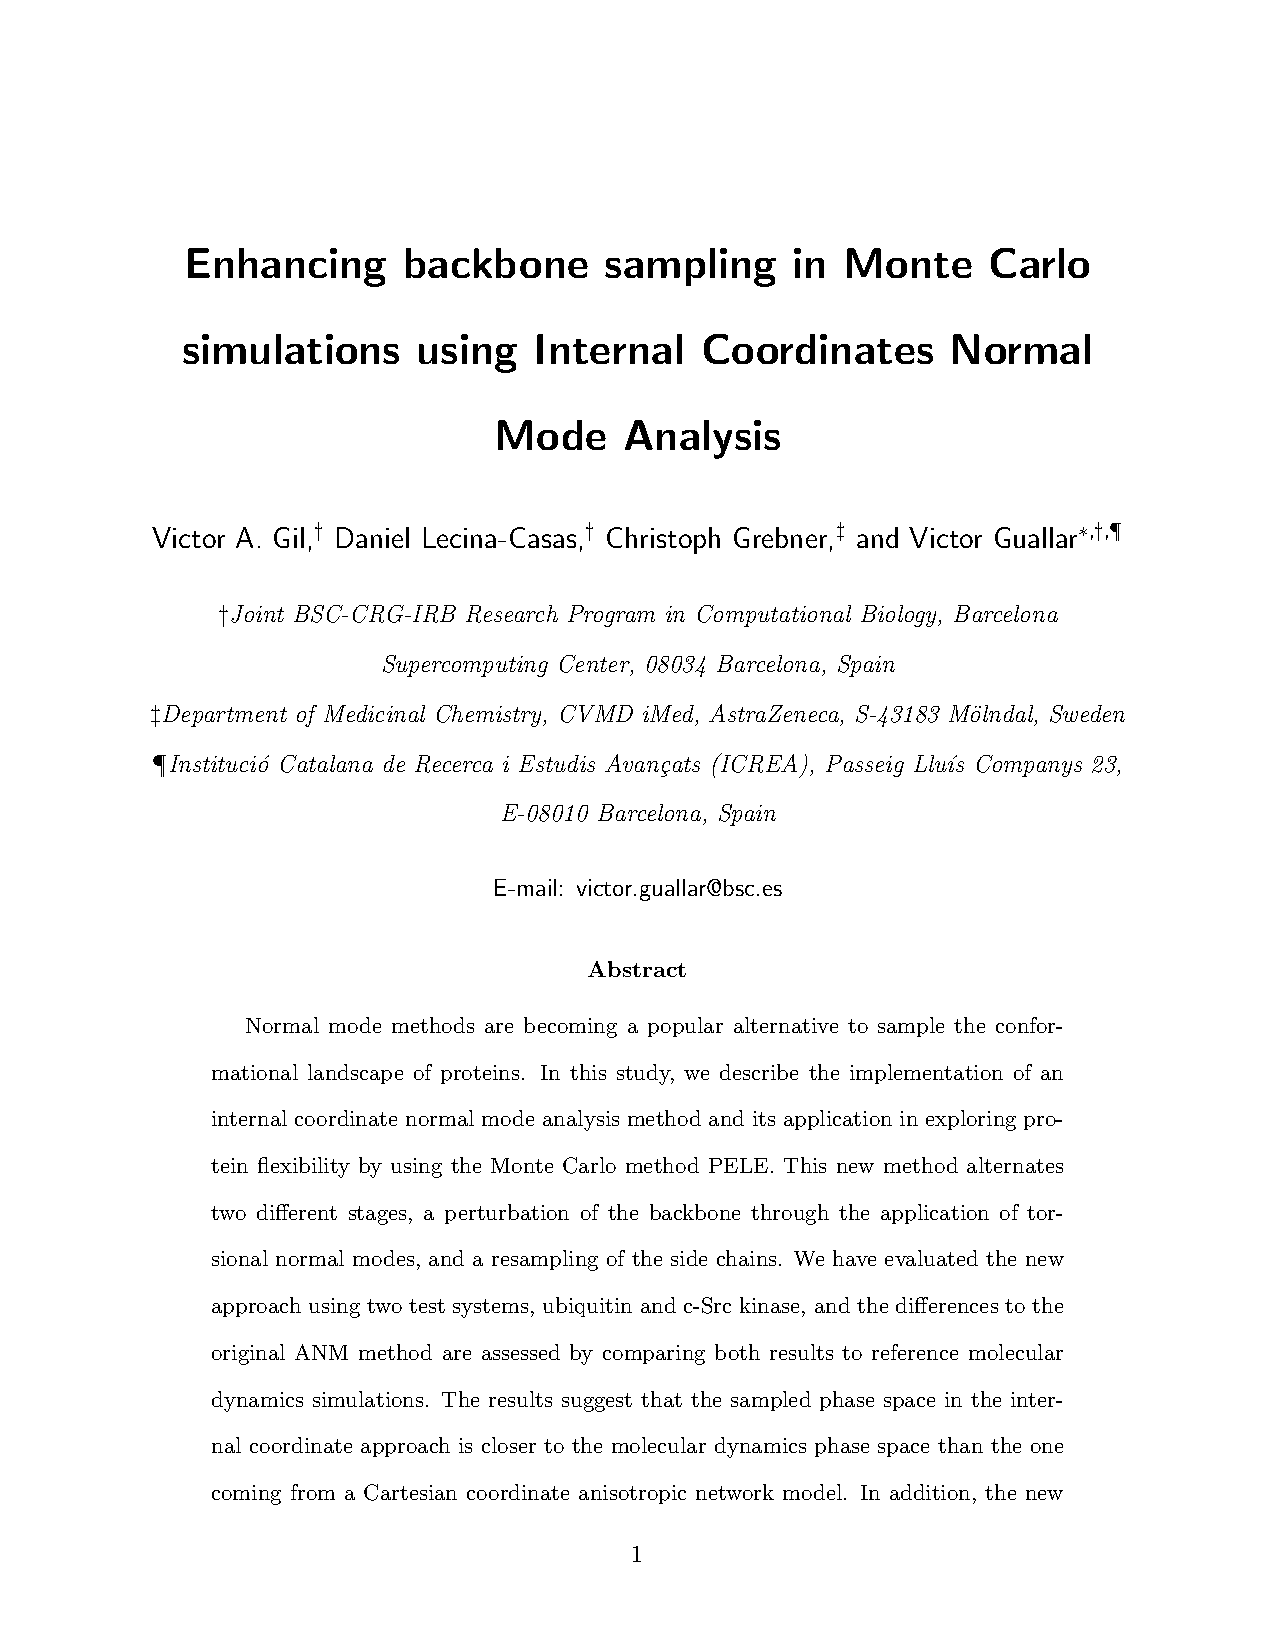
\includepdf[pages=-]{icnma.pdf}
\newpage
\cleardoublepage
\section[Supplementary materials: Enhancing sampling]{Supplementary materials for: Enhancing backbone sampling in Monte Carlo simulations using Internal Coordinates Normal Mode Analysis}

\subsection[Are CC and IC modes equivalent?]{Are Cartesian coordinate and internal coordinate normal modes equivalent?}
\label{sec:supp_mat_cc_vs_c}
We have calculated the (Cartesian coordinate) ANM modes and the internal coordinates NMA modes of a set of structures and compared them. Our test set comprises the proteins with PDB ID: 1ubq, 2lzm, 1ex6, 1ddt, 4ake, 1ggg, and the src kinase domain of 1y57. Most of these proteins have been used in NMA benchmarks, as they present wide inter domain movements. We have added two alternative structures for 1ubq and 1y57: 1ubq\_cut, a copy of 1ubq that does not contain the last 3 residues from the C-terminal loop and 1y57\_MD, a randomly picked frame from an MD simulation of 1y57.

The first thing needed in order to compare both sets of modes is to convert the IC modes to CC modes. This can be achieved calculating the Jacobian (J, inverse of Wilson's $B$ matrix) as
\begin{equation}
J_{i,\alpha} = \frac{\partial r_i}{\partial q_\alpha},
\end{equation}
and applying the following equation:
 \begin{equation}
\Delta \vec{r}_{i,\alpha} = \sum_{\alpha}^N \vec{J}_{i,\alpha} v_i^\alpha .
\end{equation}
As all heavy atoms are involved in the calculation of the IC modes and in the conversion, the resulting CC modes will have 3H elements (being H the number of heavy atoms). 

\subsubsection{Collectivity of CC and IC modes}
One of the most compelling features of NMA-based protein simulations is that the modes of lower frequency are able to mobilize big groups of atoms that perform large displacements (i.e. large collective motions). It would be interesting to know if this assumption is true for both models, and if the performance of both is similar. In order to do this we have calculated the first ten ANM and IC NMA modes for and all the structures in our test, modifying the cutoff distance that modulates the density of springs in the elastic network. Then, we have calculated the degree of collectivity of each mode. This gives us information about how the modes change when the elastic network and the shape of the protein change. 

We have also performed a second batch of calculations of IC modes applying the method described by Lu \textit{et al.} \cite{lu_new_2006}. In his work, they add an extra term to the NMA potential, $\nicefrac{\omega}{2} \sum_\alpha (\phi_\alpha - \phi_{\alpha}^0)^2$, where $\omega = 3 min(H_{\alpha\alpha}^0) $. This extra term modifies the Hessian diagonal, presumably lowering the so-called ``tip effect'' problem.

To quantify the differences of collectivity, we will calculate the degree of collectivity. This measure, first proposed by Bruschweiler \cite{bruschweiler_collective_1995}, quantifies the number of atoms that are affected by a mode and the relative magnitude of the induced displacement. Its value can be calculated as

\begin{equation}
\kappa_i = \frac{1}{N} exp \left( -\sum^N_j \alpha \Delta R_j^2 log \left( \alpha \Delta R_j^2 \right) \right),
\end{equation}

where $N$ is the number of atoms and $\Delta R_j$ is the atomic displacement described by mode $i$ on atom $j$. 
The degree of collectivity is proportional to the exponential of the ``information entropy'' embedded in vector $\Delta R$ \cite{tama_conformational_2001}. Its lower and upper bound is known ($N^{-1}$ and 1 respectively). This allows us to normalize its value in the range $[0,1]$, meaning 1 that the conformational change the mode produces is maximally collective.

As we can see in Fig. \ref{fig:collectivities_per_cutoff}, the average collectivities of the CC modes are always lower than their IC counterparts. Furthermore, the degree of collectivity seems to decline as the cutoff varies and the elastic network becomes more dense. Conversely, the IC modes remain almost unaffected by the changes of the elastic network. It is worth noting that the ones calculated using the Hessian modification method have slightly higher values of collectivity and are, again, almost immune to the EN changes. 

\begin{figure}
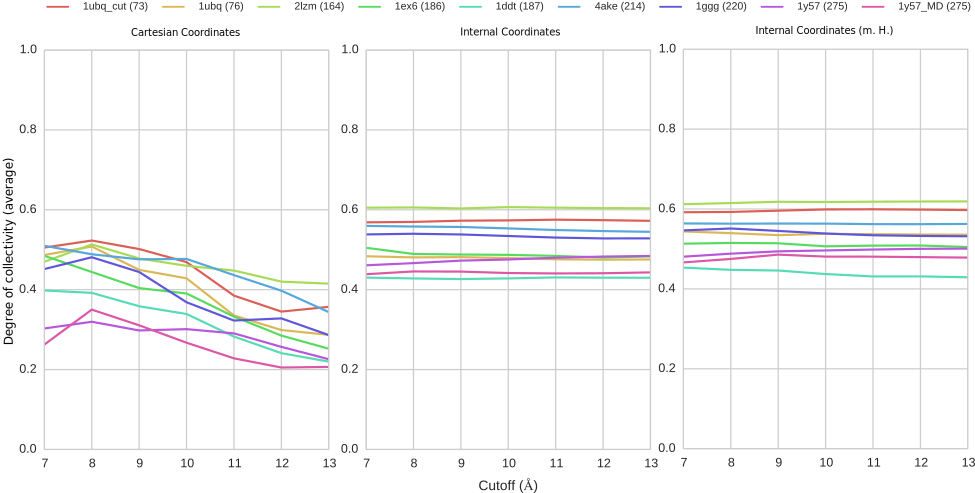
\includegraphics[width=\linewidth, height=\textheight, keepaspectratio]{avg_collectivities_per_cutoff}
\caption{Degree of collectivity for each structure and calculation method. .}
\label{fig:collectivities_per_cutoff}
\end{figure}

From the plot we can see that 9 $\AA$ is a good choice for the cutoff: it yields good collectivity values and it is in agreement with the conclusions of other studies \cite{zheng_anharmonic_2010}.

\begin{figure}
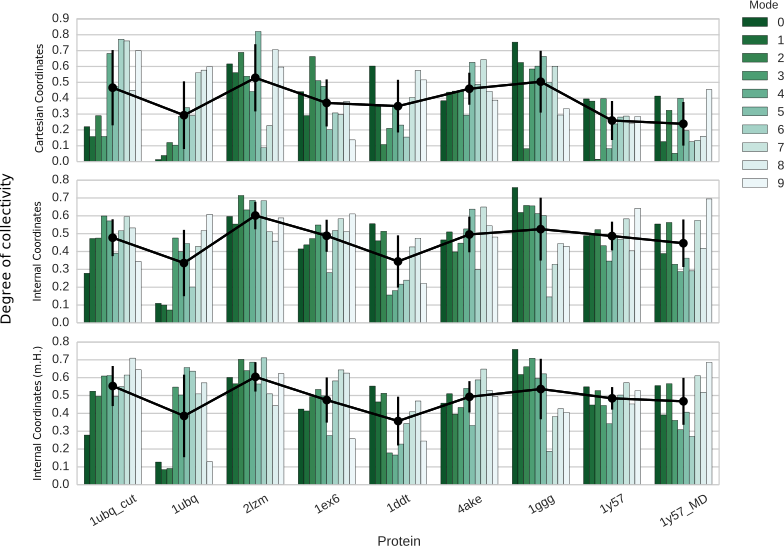
\includegraphics[width=\linewidth, height=\textheight, keepaspectratio]{cut_9_avg_coll}
\caption{Detailed study of the degree of collectivity per mode, structure and method. Cutoff has been set to 9 \angstrom. The Hessian modification method (m.H.) produces only slight improvements, generally concentrated in higher frequency modes.}
\label{fig:cut_9_avg_coll}
\end{figure}

The detailed view of mode collectivities for a cutoff of 9 \angstrom  is shown in Fig. \ref{fig:cut_9_avg_coll}. We can see how the collectivity of IC modes is higher, especially that of the lower frequency modes. The differences between 1ubq\_cut and 1ubq are of particular interest. In these two cases, the collectivity values of the lower frequency modes of 1ubq are pretty small for all three methods, and they increase perceptibly in 1ubq\_cut. This must be caused by the only difference between these two structures: the appearance of the C-terminal loop. The structure with the loop (1ubq) is severely suffering from the ``tip effect'' due to the flexibility of the final loop, perfectly illustrating how this effect can worsen the collectivity of the modes.  

From the analyses performed on this data set, we can conclude that IC modes have higher collectivity, and  that this collectivity is more robust to changes in the elastic network.  

\subsubsection{Comparison between the CC and IC mode spaces}

We also wonder to which extent the mode space spanned by the CC and IC modes is similar. To this end we will use two measures: the cumulative overlap and the root mean square inner product (RMSIP). Both of them are based on the mode overlap operation, which measures the projection of one mode over the other. It can be calculated as:
\begin{equation}
O_{ij} = \frac{\left | P_i . M_j \right |}{{\Arrowvert P_i\Arrowvert}{\Arrowvert M_j\Arrowvert}} .
\end{equation}
Its value ranges from 0 to 1, meaning 1 a perfect overlap.  

The Cumulative overlap \cite{yang_close_2008} measures to which extent a range of modes can capture the motion of a single mode. It is calculated as
\begin{equation}
CO_i(k)= (\sum_{j}^{k} O_{ij}^2)^\frac{1}{2},
\end{equation}
where $i$ is the mode we are checking and $[j,k]$ is the range of modes we will use to explain the first. Its value is, again, in the range from 0 to 1, meaning 1 a perfect match (assuming perfect orthogonality of the modes).   

Finally, the RMSIP \cite{amadei_convergence_1999,leo-macias_analysis_2005} measures how the normal mode space spanned by a range of modes overlaps with another range of modes. It is calculated as  
\begin{equation}
RMSIP(l,m) = \left( \frac{1}{l} \sum_{i=1}^l \sum_{j=1}^m {(P_i.M_j)}^2 \right )^\frac{1}{2} .
\end{equation}
Its value is independent of the mode order and ranges from 0 to 1, meaning 1 that both normal mode spaces are identical.

It is important to note that the modes coming from the IC conversion and PELE ANM model are defined for a different number of atoms (all heavy atoms in the first case, $C_\alpha$s in the second) and, therefore, they represent very different mode spaces. In order to make the comparisons possible, we need to calculate the ANM modes for all heavy atoms.

The cumulative overlaps shown in Figs. \ref{fig:avg_cum_overlap_per_cutoff} and \ref{fig:cut_9_cumulative_overlap} indicate that both mode spaces can explain each other successfully, being 1ubq, 1ubq\_cut and 1y57\_MD the only exceptions. In general, increasing the cutoff makes the differences between mode spaces more noticeable. The calculations performed with cutoff distance equal to 9 \angstrom (Fig. \ref{fig:cut_9_cumulative_overlap}), show that lower frequency modes are generally the ones that find a best correspondence with the modes of the other space.

\begin{figure}
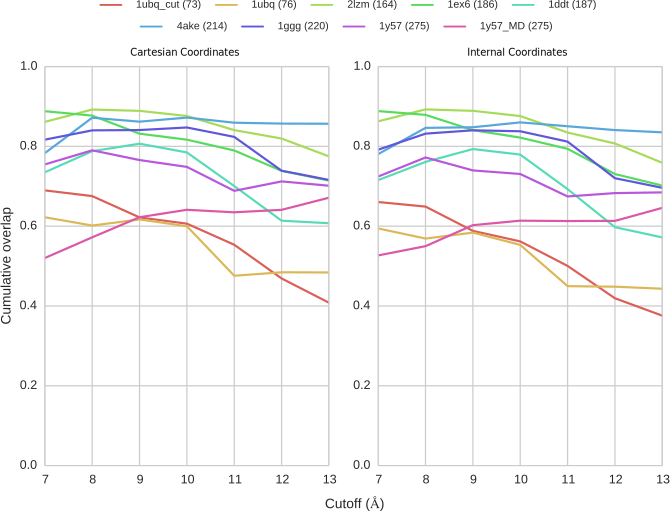
\includegraphics[width=\linewidth, height=\textheight, keepaspectratio]{avg_cum_overlap_per_cutoff}
\caption{ Average cumulative overlap for different cutoff distances, methods, and structures in our test set. Standard deviations are not shown for the sake of clarity.}
\label{fig:avg_cum_overlap_per_cutoff}
\end{figure}
 
\begin{figure}
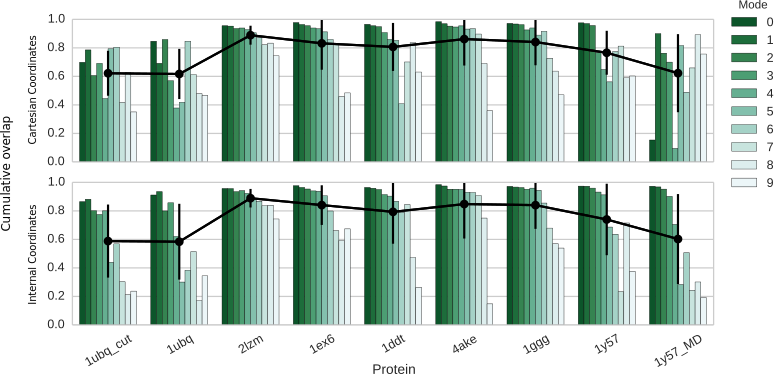
\includegraphics[width=\linewidth, height=\textheight, keepaspectratio]{cut_9_cumulative_overlap}
\caption{Detailed study of the cumulative overlap per mode, structure and method. Cutoff has been set to 9 \angstrom. In general, the rightmost modes (higher frequencies) are the ones with worst overlap.} 
\label{fig:cut_9_cumulative_overlap}
\end{figure}

Regarding the RMSIP for the modes calculated using a cutoff distance of 9 \angstrom, the mode space overlap is higher for the subspace of the low frequency modes, and decreases when more high frequency modes are added to the calculation (see Fig. \ref{fig:cut_9_rmsip_per_mode_range}), which correlates well with the observations made for Fig. \ref{fig:cut_9_cumulative_overlap}.

\begin{figure}
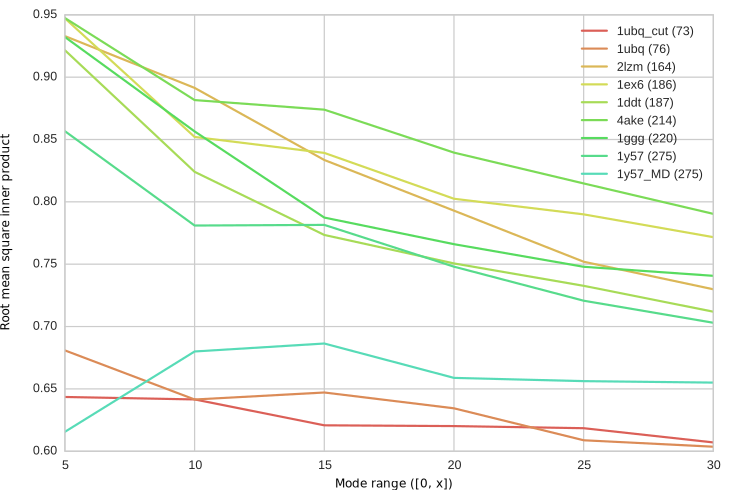
\includegraphics[width=\linewidth, height=\textheight, keepaspectratio]{cut_9_rmsip_per_mode_range}
\caption{RMSIP of CC and IC mode spaces. The x-axis shows the upper limit of the mode space tested (e.g, 10 means that the first ten modes are to be used to obtain the RMSIP). Both spaces look to be very similar, at least for the 5 lowest frequency modes. The similarities decrease as we move to modes of higher frequencies, with the only exceptions already commented in the cumulative overlap study.}
\label{fig:cut_9_rmsip_per_mode_range}
\end{figure}

\newpage
\cleardoublepage

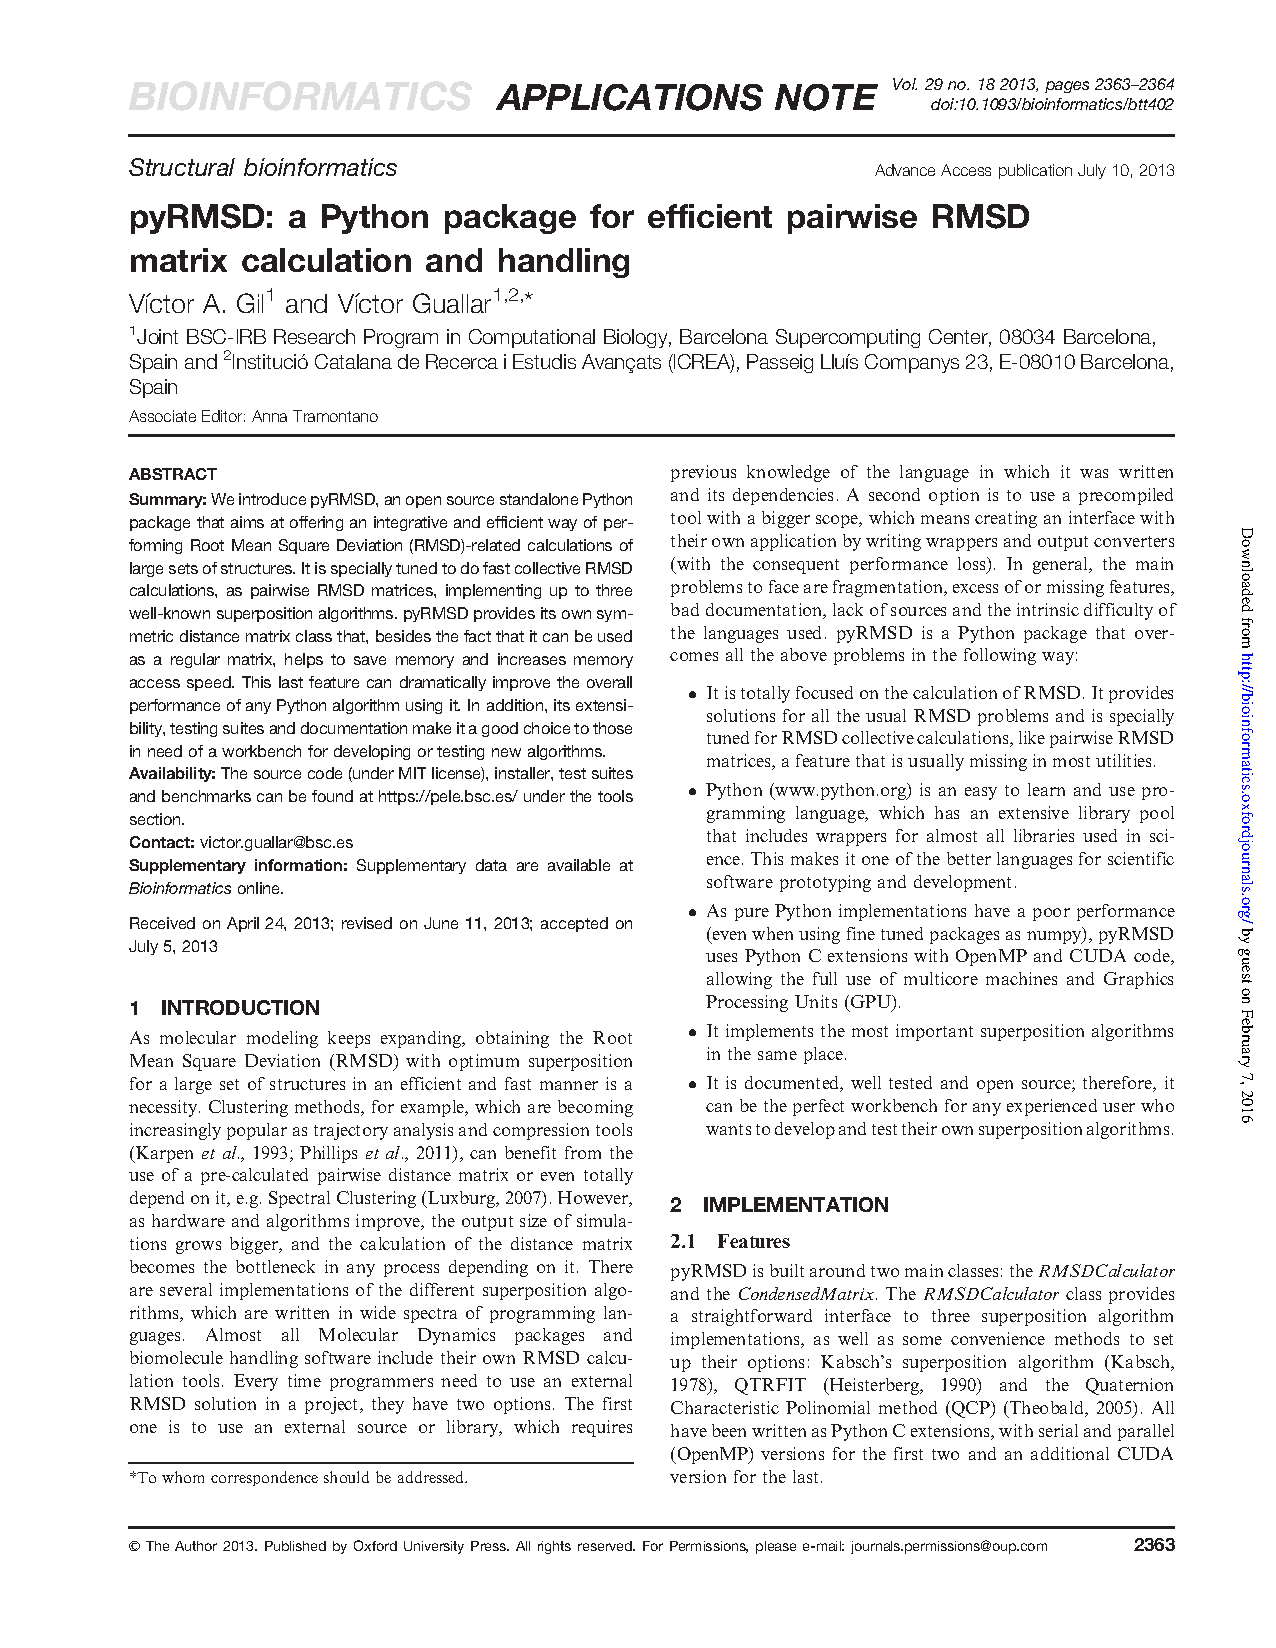
\includepdf[pages=-]{pyrmsd.pdf}
\newpage
\cleardoublepage
\section[Supplementary materials: pyRMSD]{Supplementary materials for: pyRMSD: a Python package for efficient pairwise RMSD matrix calculation and
handling}

Comparing the performance of different algorithms is not straightforward. We can deduce some theoretical bounds,
but these might be too general to have any practical value, especially when comparing similar algorithms. When this
happens, the only way to go is to compare implementations.

In our implementations, good code design (especially reusability) had a bigger priority than optimality. All three
algorithm implementations have been coded sharing the same framework, reusing as many pieces of code as possible. This
enhances the comparability of our implementations, which may be suboptimal in the same degree, giving us a unique
opportunity of making a more fair performance comparison between them.

All benchmark tests were performed in BSC's Minotauro \cite{barcelona_supercomputing_center_minotauro_2015}, which has been built with Intel Xeon E5649 CPUs and NVIDIA M2090
GPUs. Only 1 GPU was reserved for CUDA runs. OpenMP runs used six threads at most.

\subsection{Algorithm performance comparison}
In order to get a good overview of each algorithm{}'s performance, we have checked the time that each of the three
algorithms need to complete the execution of each one of pyRMSD's basic methods (oneVsFollowing, pairwiseMatrix and
iterativeSuperposition). A 30k trajectory of Ubiquitin (reading only \calpha atoms) was used. The oneVsFollowing method has
been tested without and with input coordinates rotation, as this last adds overhead to QCP implementation due to the
mandatory rotation matrix calculation (QCP does not need to calculate it otherwise).

For basic linear operations (see Fig.~\ref{fig:pyrmsd_supp:1}), QCP has the best performance of all three, even when the rotation matrix is
calculated (oneVsFollowing(r) and iterativeSuperposition). The use of OpenMP smooths differences so much that choosing
one algorithm over the other becomes a mere matter of preference (see Fig.~\ref{fig:pyrmsd_supp:2}).

\begin{figure}
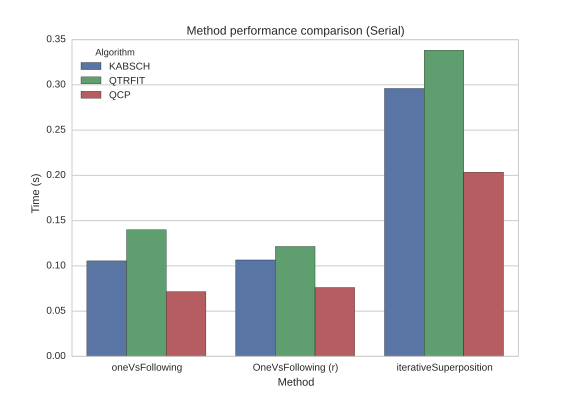
\includegraphics[width=\linewidth,height=\textheight,keepaspectratio]{pyrmsd_supp_serial_method_perf_comp.pdf}
\caption{ Comparison of the execution of three methods for the three available algorithm
implementations (serial).}
\label{fig:pyrmsd_supp:1}
\end{figure}

\begin{figure}
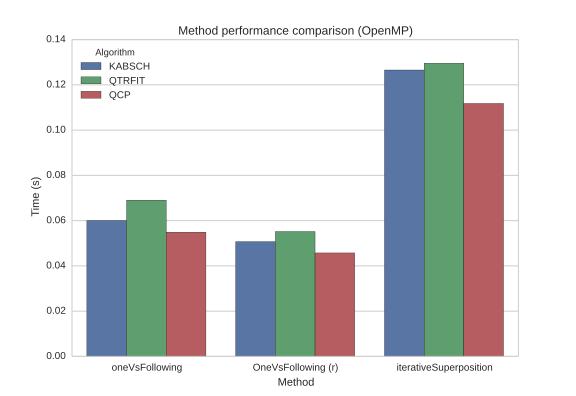
\includegraphics[width=\linewidth,height=\textheight,keepaspectratio]{pyrmsd_supp_openmp_method_perf_comp.pdf}
\caption{ Comparison of the execution of three methods for the three available algorithm
implementations (OpenMP).}
\label{fig:pyrmsd_supp:2}
\end{figure}

However, things change when comparing the performance of the pairwise matrix generation (see Fig.~\ref{fig:pyrmsd_supp:3}). Small performance
differences get amplified because of the quadratic nature of the problem. In this case, we observe that QCP excels by
achieving a 2x/4x speedup with respect to the other two, in both serial and OpenMP modes.

\begin{figure}
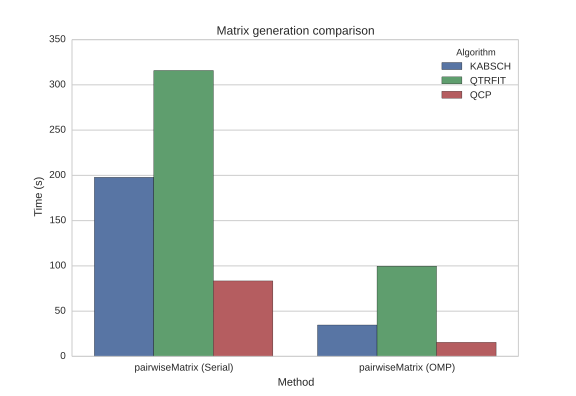
\includegraphics[width=\linewidth,height=\textheight,keepaspectratio]{pyrmsd_supp_matrix_gen_comp.pdf}
\caption{ Calculation time of a pairwise matrix from a 30k frames trajectory.} 
\label{fig:pyrmsd_supp:3}
\end{figure}

\subsection{QCP performance}
We want to compare all four implementations of QCP algorithm: serial, OpenMP, CUDA and CUDA with full matrix memory
allocation into the device. To this end, we will use the pairwiseMatrix method over Ubiquitin trajectories of 5, 10, 15,
20, 25, 30 and 35k frames.

We can see in the resulting plot (Fig.~\ref{fig:pyrmsd_supp:4}) that OpenMP version is about 5x faster than the serial one, and CUDA version
is about 8,5x faster.

\begin{figure}
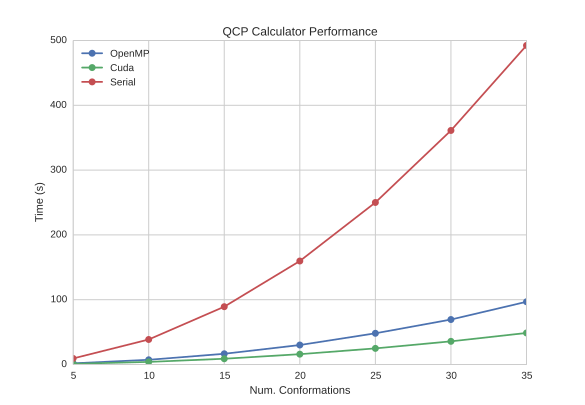
\includegraphics[width=\linewidth,height=\textheight,keepaspectratio]{pyrmsd_supp_qcp_perform_1.pdf}
\caption{ Performance comparison of serial, OpenMP and CUDA (single-precision) implementations of the QCP algorithm.}
\label{fig:pyrmsd_supp:4}
\end{figure}

After profiling the CUDA version, we saw that a considerable part of the time was spent in memory transactions from the
device to the host. The RMSD matrix is calculated line by line and, after each one of this calculations, the host
matrix representation is updated. This method can be successfully used in a broad range of GPUs, as it does not require
cards with big amounts of RAM. We implemented another method that holds the entire matrix in GPU's RAM. The speedup is
greater (11x compared with serial code), as memory transactions are performed only once (Fig.~\ref{fig:pyrmsd_supp:5}).

\begin{figure}
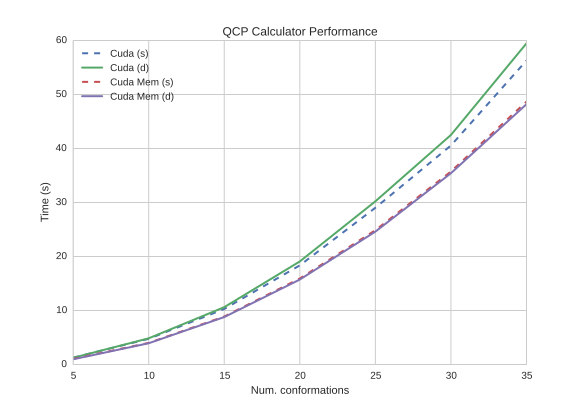
\includegraphics[width=\linewidth,height=\textheight,keepaspectratio]{pyrmsd_supp_qcp_perform_2.pdf}
\caption{ Performance comparison of CUDA implementations. 'Mem' versions hold the entire
matrix into memory, (s) versions use single-precision arrays and (d) versions use double-precision arrays.}
\label{fig:pyrmsd_supp:5}
\end{figure}

Finally, there are two things worth mentioning. The first one is that our CUDA implementation can be further improved by
enhancing work balance and memory coalescence. The second is that the use of single point precision in our QCP CUDA
implementation, contrary to what is expected, does not perform substantially better than the double precision
implementation. The reason for this behavior is again the big effort put into generalizing the code. pyRMSD uses
internally double-precision arrays to store coordinates and RMSD values. This implies that, when using GPUs without
double-precision support, a single-precision temporary buffer is to be filled at every host to device memory move.

\subsection{Input size response of \ QCP implementation}
The last benchmark established a clear relationship between the size of a trajectory (in frames) and the time needed to
do calculations. In this benchmark we want to fix the number of frames and test the impact of biomolecule sizes in
performance. The number of frames of the trajectory will be 10k, and the number of atoms of each one of the conformers
will be artificially increased at every step in order to calculate the pairwise RMSD matrix.

Both CUDA and OpenMP implementations, show a linear increase of the time needed to calculate the matrix (Fig.~\ref{fig:pyrmsd_supp:6}).
Incrementing conformer size does not increase or decrease performance.

\begin{figure}
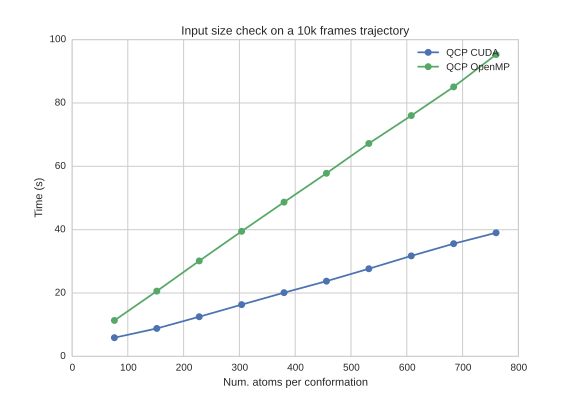
\includegraphics[width=\linewidth,height=\textheight,keepaspectratio]{pyrmsd_supp_input_size_check.pdf}
\caption{ Input size response of the OpenMP and CUDA versions of the QCP algorithm.}
\label{fig:pyrmsd_supp:6}
\end{figure}

\subsection{Accuracy check}
While KABSCH algorithm tries to find an optimal rotation matrix, QTRFIT and QCP will use quaternions in order to get
this rotation. Does the base method affect accuracy? In this test, we have applied the oneVsFollowing method over the
first frame of a 10k frames Ubiquitin trajectory. Then we have calculated the root mean square of the differences,
which will be our index of RMSD value variation. 

In Table \ref{tab:pyrmsd_supp:rmsd_accuracy}, we can see that all implementations have an RMS different than 0, which means that all algorithms have
calculated different RMSD values. Kabsch's algorithm and QTRFIT have close results in spite of their different
approaches to calculating the superposition. QCP CUDA single-precision floating point version differs the most, being the
double-precision version the most accurate of both.

\begin{table}
\centering
\begin{tabular}{ c c c c c c } 

\toprule
Method & KABSCH & QTRFIT & QCP & \specialcell{QCP CUDA\\(Single)} & \specialcell{QCP CUDA\\(Double)}\\
\midrule

KABSCH & ~ & 2.308e-12 & 2.678e-12 & 1.028e-03 & 2.689e-12\\
QTRFIT & ~ & ~ & 1.568e-12 & 1.028e-03 & 1.547e-12 \\
QCP & ~ & ~ & ~ & 1.028e-03 & 8.926e-13\\
\bottomrule

\end{tabular}
\caption{Root Mean Square of the RMSD array differences for each of the algorithms.}
\label{tab:pyrmsd_supp:rmsd_accuracy}
\end{table}

It is important to note that, although QCP solves the problems of prior methods like Diamond's \cite{diamond_note_1988} algorithm instability in
rotations close to 180�, it can suffer from convergence problems derived from the use of Newton-Raphson root-finding
method.

However, differences are generally small, and RMSD is often used qualitatively, which means that, unless we require high
precisions, all algorithm implementations are interchangeable.

\subsection{OpenMP scalability}
We want to study the scalability of the OpenMP version of each of the algorithms. To achieve it we have calculated the
pairwise RMSD matrix of a 30k frames trajectory of Ubiquitin, using a different number of threads for each execution
(from 1 to 6).

It is not difficult to see that we obtain a linear speedup, with a maximum of 5.6-5.8x for six threads (compared with the
one thread run), which is close to the theoretical maximum speedup (6x for six threads) (Fig.~\ref{fig:pyrmsd_supp:7}, \ref{fig:pyrmsd_supp:8}).

\begin{figure}
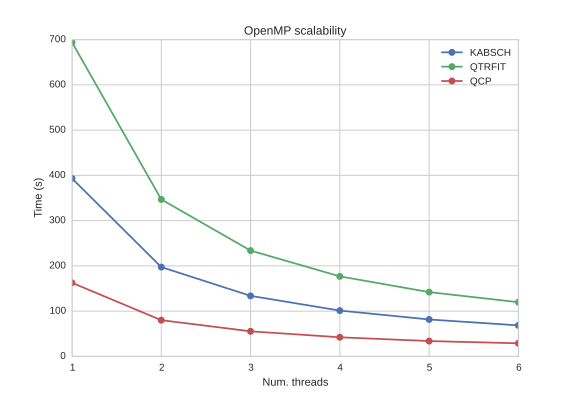
\includegraphics[width=\linewidth,height=\textheight,keepaspectratio]{pyrmsd_supp_omp_scalability.pdf}
\caption{ Time needed to compute a pairwise matrix from a 30k frames trajectory using a
different number of threads.}
\label{fig:pyrmsd_supp:7}
\end{figure}

\begin{figure}
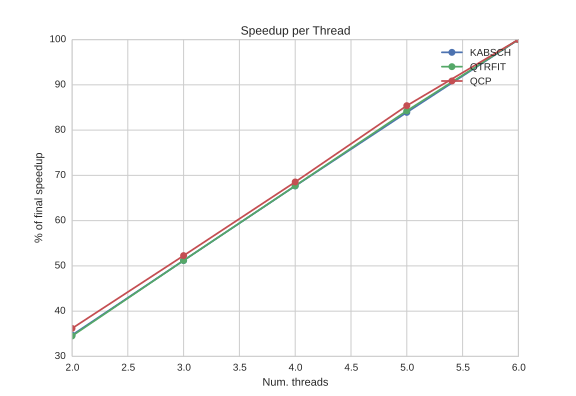
\includegraphics[width=\linewidth,height=\textheight,keepaspectratio]{pyrmsd_supp_speedup_per_thread.pdf}
\caption{ Percentage of speedup per thread added to the calculation. Speedup is almost
linear with number of threads.}
\label{fig:pyrmsd_supp:8}
\end{figure}

\subsection{Comparison with existing packages}
As a final test, we will compare pyRMSD with other software packages that include RMSD calculation features. We have
chosen four publicly available open source packages:

\begin{description}
	\item [g\_rms]  Is a C-written command line program part of the Gromacs \cite{berendsen_gromacs_1995} suite. Its main feature is the fast creation of
	distance matrices from trajectories.
	\item [Prody \cite{bakan_prody_2011-2}] A Python package which offers very interesting features to load and analyze biomolecule trajectories,
	including a complete PDB parser and a powerful selection language.
	\item [Biopython \cite{cock_biopython_2009-1}] A mature Python package which offers numerous bioinformatic computational tools.
	\item [PyVib2 \cite{fedorovsky_pyvib2_2007}] A pure Python package used to analyze vibrational motion and spectra of molecules.
\end{description}

Our comparison will be based on two measures: calculation time and integration complexity. To this aim we have created 4
scripts \footnote{The scripts can be found in \url{https://github.com/victor-gil-sepulveda/pyRMSD-Comparison.git}}. 
Every script calculates the RMSD
matrix of a trajectory twice, first using one of the aforementioned packages, and then replicating the same calculation
using pyRMSD (serial). Integration complexity has been measured as the ratio between the number of effective code lines
necessary to program the task with the tested package and pyRMSD. Performance has been calculated as the ratio of the time
needed to complete the task by the tested package over the time required by pyRMSD. All tests were performed on a workstation 
with an Intel Xeon W3530 CPU (four cores at 2.80GHz) with 12GB of RAM. 

\begin{sidewaystable}
\caption{Comparison of the time, lines of code, speedup and integration complexity (I.C.) needed to complete an RMSD collective operation.}
\centering
\begin{center}
\begin{tabular}{ r r c c c c c c }
\toprule
Method & Frames & Time (s) & Time pyRMSD(s)& 
 Lines of code & Lines of code (pyRMSD) & Speedup & I. C. \\ 
\midrule

\textbf{g\_rms} & 10 & 0.0564 & 0.0466 & 24 & 3 & 1.21 & 8 \\ 
~ & 100 & 0.7421 & 0.488 & ~ & ~ & 1.52 & ~ \\ 
~ & 1000 & 62.5245 & 14.6778 & ~ & ~ & 4.26 & ~ \\ 
\textbf{Prody} & 10 & 0.1698 & 0.0008 & 6 & 1 & 212.25 & 6 \\ 
~ & 100 & 3.408 & 0.0587 & ~ & ~ & 58.06 & ~ \\ 
~ & 1000 & 312.7806 & 6.0187 & ~ & ~ & 51.97 & ~ \\ 
\textbf{PyVib2} & 10 & 4.069 & 0.0001 & 7 & 1 & 40690.00 & 7 \\ 
~ & 100 & 450.1247 & 0.0995 & ~ & ~ & 4523.87 & ~ \\
~ & 1000 & 30332.6163 & 10.372 & ~ & ~ & 2924.47 & ~ \\ 
\textbf{Biopython} & 10 & 2.012 & 0.0008 & 8 & 1 & 2515.00 & 8 \\ 
~ & 100 & 219.6425 & 0.0572 & ~ & ~ & 3839.90 & ~ \\ 
~ & 1000 & 22003.5187 & 6.0966 & ~ & ~ & 3609.15 & ~ \\ 

\bottomrule
\end{tabular}
\end{center}
\label{tab:pyrmsd_supp:speedup}
\end{sidewaystable}

Table \ref{tab:pyrmsd_supp:speedup} shows that pyRMSD is always faster than the other packages. In the last three cases, this is because
that RMSD calculations are also written in pure python (which includes the use of numpy), while in pyRMSD these have
been written as C extensions. These packages have not been specifically designed to handle RMSD collective operations,
which explains why more lines of code are needed. Biopython and PyVib2 RMSD-related features are indeed constrained to
the pairwise RMSD case, while Prody can calculate rows of the matrix using only one function. This makes the last
faster and easier to use in this scenario. g\_rms is considerably faster than the others, as it has been written in C
and because of its narrower scope. However, to use it within a Python script, the user will need to create a wrapper to
control the program execution (here simplified by the utilization of the `expect' command), and a method to parse program
results. This adds extra complexity to the code as well as a performance penalty.







\newpage
\cleardoublepage

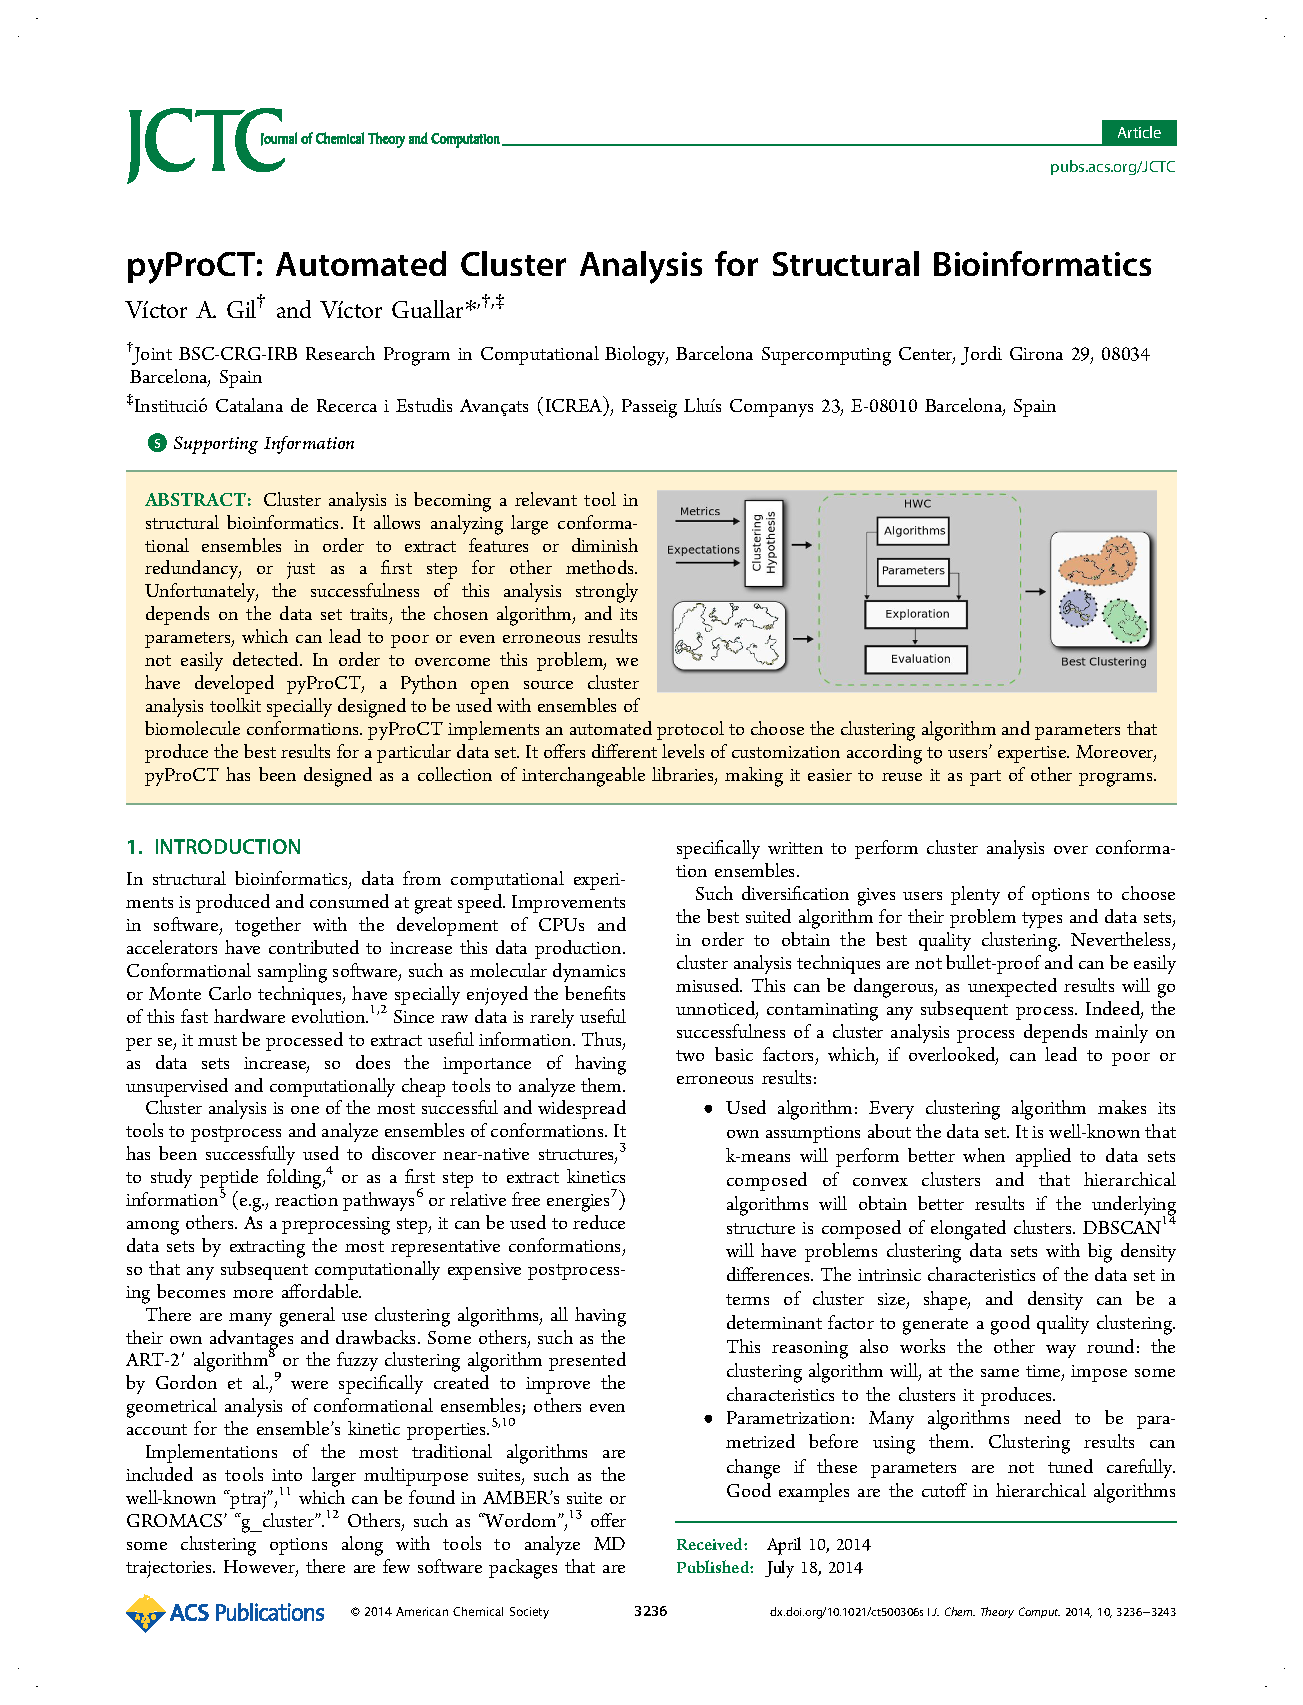
\includepdf[pages=-]{pyproct.pdf}
\newpage
\cleardoublepage
\section[Supplementary materials: pyProCT]{Supplementary materials for: pyProCT: Automated Cluster Analysis for Structural Bioinformatics}
\subsection{Implemented clustering algorithms}

In this section, we will review the algorithms currently implemented
in pyProCT. For each of these, we will briefly describe how it works,
how its parameters are generated (if automatic generation is triggered)
and the structure of each parameter objects, so that users can define
them inside the script.


\subsubsection[DBSCAN]{DBSCAN \cite{ester_density-based_1996}}

DBSCAN\footnote{Density-Based Spatial Clustering of Applications with Noise} 
is a density-based clustering algorithm. Density is given by the use
of 2 parameters: `eps', that defines a distance radius centered on
one element, and `minpts', that specifies the minimum number of neighboring
points for that element to be considered part of a cluster. 

The algorithm classifies elements into three categories: not classified,
noise and core elements. All elements are initially set to `not classified'.
The `core' elements are those that have at least `minpts' elements
in an `eps' radius and also the elements inside the `eps' radius of
a `core' element (which will be border points). All not `core' elements
are classified as 'noise' and will not be part of the clustering. 

One of the key issues of DBSCAN is the proper selection of its 'eps'
and `minpts' parameters. High density combinations can produce very
noisy clusterings (which, depending on the context can be an issue
or a feature), and low density combinations can easily lead to the
singleton clustering (a clustering with only one cluster encompassing
all elements). Because of its dependency on the element density, it
can have problems detecting clusters if there are different density
regions in the dataset.


\subsubsubsection{Parameters generation strategy} 

The implemented parameters generator is based on the details given
in the original articles \cite{ester_density-based_1996, sander_density-based_1998-2}
as well as the method of Ankerst 	extit{et al.} \cite{ankerst_optics_1999-1}.
Briefly: 

\begin{enumerate}
\item pyProCT will recreate k-distance lists for some k values ( 
$ k < \log \left ( \abs{D} \right )$ 
as indicated in the literature). 

\item For each of the k-distance lists, an `eps' value will be chosen so
that the generated noise falls between 0\% and the maximum allowed
noise (plus a 2.5\% margin). The value of k in that k-distance list
will be used as the value of `minpts' in that parameter pair. 
\end{enumerate}

In addition, we add the parameter choice suggested by Zhou 	extit{et al.}\cite{zhou_research_2012-1}.


\subsubsubsection{Parameters object structure }
\begin{lstlisting}[language=json,firstnumber=1] 
{ 	
	"eps": Real,
	"minpts": Integer 
}
\end{lstlisting}


\subsubsection{GROMOS}

First found in the work of Daura 	extit{et al.} \cite{daura_peptide_1999,daura_folding-unfolding_1999-1},
it is also a density-based algorithm. As it looks that the algorithm
has no name, we named it after the flag that the g\_cluster tool\cite{berendsen_gromacs_1995}
receives to use it. With a simpler behaviour than DBSCAN, it was thought
to adapt to the ideal expected characteristics of datasets coming
from the conformational search of small peptides (well-separated regions
centered in metastable states). 

The algorithm repeats a loop that ends when all elements have been
clustered:

\begin{algorithm}[H]
\caption{GROMOS algorithm}
\begin{algorithmic}[1]
\Input $D$, the data set
\Input $cutoff$, the cutoff radius
\Output $C$, a set of clusters
\State $D_{tmp} \gets D$ \;
\While{ $D_{tmp} \neq \emptyset$}
\State $e \gets$ mostDense($D_{tmp}$)\;
\State $neig \gets$ neighbours($e$,$cutoff$)\;
\State $c \gets \{e, neig\}$\;
\State addCluster($c$, $C$)\;
\State $D_{tmp} \gets D_{tmp} \setminus c$\;
\EndWhile
\State \textbf{return} C
\end{algorithmic}
\end{algorithm}

\begin{description}
\item [mostDense()] Find the element with more neighbors inside the given cutoff radius
(to find the densest zone). 
\end{description}

\subsubsubsection{Parameters generation strategy}

The goal here is to find a finite range of cutoffs, exactly as it is done with
the `k' parameter in k-medoids or `num\_clusters' in the random grouping
algorithm. The minimum value for the cutoff parameter is 0, generating
a trivial clustering in this case (a clustering where each element
is a cluster). In order to get an estimation of the maximum value,
we choose the 3 most separated elements of the dataset. We can ensure
that the second longest side of the triangle with this 3 elements
as vertices will be the minimum radius that encompasses all elements
of the dataset, producing a singleton clustering, and thus it is the
upper limit of the cutoff range. Once the maximum and minimum are
known, we can obtain equidistant values for the cutoff within this
range.


\subsubsubsection{Parameters object structure}
\begin{lstlisting}[language=json,firstnumber=1] 
{ 	
	"cutoff": Real
}
\end{lstlisting}


\subsubsection{Hierarchical clustering}

pyProCT uses an external package \cite{mullner_fastcluster_2013}
that implements an agglomerative hierarchical clustering algorithm.
Agglomerative hierarchical algorithms start with all elements of the
dataset forming single clusters (a trivial clustering) and every step
it merges the closest clusters by means of a proximity function (only
`single linkage' and `complete linkage' options can be used). The
agglomerative step represents the dataset as a tree (dendrogram) that
has to be cut in order to retrieve the clustering. The distance at
which the cut is performed is called the cutoff distance.


\subsubsubsection{Parameters generation strategy}

Getting the dendogram cut is computationally cheap compared to the
hierarchical matrix calculation. In this case, pyProCT will generate
clusterings until it finds the range of cutoffs in which the resulting
clustering falls within the range of allowed number of clusters. This
range will be refined in order to get more clustering candidates.


\subsubsubsection{Parameters object structure}
\begin{lstlisting}[language=json, firstnumber=1] 
{ 	
	"cutoff": Real, 
	"method": String in ["single", 
			   "complete"] 
}
\end{lstlisting}
\begin{description}
\item [method] If its value is `single', the single linkage method
is used to calculate the proximity of clusters. This proximity is
then defined as the minimum distance between any two points in that
clusters. If `complete' is used instead, the proximity of two clusters
is measured as the maximum distance between any two elements of different
clusters. Various combinations of method-cutoff are possible in
the parameters list, but due to performance reasons, only the `method'
value of the first parameter object in the list will be used.
\end{description}

\subsubsection{K-Medoids}

Is a partitional algorithm similar in concept to k-means. Because
of its beautiful simplicity, our implementation is based on Lloyd's
k-means algorithm \cite{lloyd_least_1982} instead that on other k-medoids
specific algorithms (like PAM \cite{kaufman_finding_1990-1}).Roughly the algorithm works as follows:

\begin{algorithm}[H]
\caption{K-Medoids algorithm}
\begin{algorithmic}[1]
\Input $k$, number of clusters
\Output $C$, a set of clusters
\State medoids $\gets$ initialSeeding(k)\;
\While{$\neg$ convergence() $~\land \neg$ maxStepsReached()}%
\State C $\gets$ labelElements()\;
\State medoids $\gets$ calculateMedoids(k)\;
\EndWhile
\State \textbf{return} C
\end{algorithmic}	
\end{algorithm}

\begin{description}
	\item[convergence()]  Checks if how the labeling of current iteration has changed with respect to the last iteration.
	\item[labelElements()] Labels each element of the dataset with the cluster of its closer medoid. 
\end{description}

K-Means-like algorithms will perform better detecting convex clusters.

\subsubsubsection{Parameters generation strategy}

A globally-defined or used-defined maximum number of parameter sets
(`max') will be generated. Each of the parameter sets will have its
`method' field set to `EQUIDISTANT' and its `k' field will is calculated as 
$(min\_clusters+step \times n$ where $0<=n<=max$ and $step$ is $\nicefrac{(max\_clusters-min\_clusters)}{max}$.

\subsubsubsection{Parameters object structure}
\begin{lstlisting}[language=json,firstnumber=1] 
{ 	
	"k": Integer, 	
	"seeding_type": String in ["RANDOM", 
			      "EQUIDISTANT", 
			           "GROMOS"], 	
	"seeding_max_cutoff": Real 
}
\end{lstlisting}

\begin{description}
	\item [k] Number of clusters to be created. 
	\item [seeding\_type] Method used for initial medoid seeding. 
	\item [seeding\_max\_cutoff] Only used when `seeding\_type' =
	GROMOS. Maximum cutoff radius for the GROMOS algorithm to generate
	the initial medoids.
\end{description}

The algorithm is very sensitive to the initial seeding configuration
(the initial placement of the medoids). Three seeding methods are
provided: 

\begin{description}
	\item [RANDOM] Uses a random choice of elements from the dataset
	as initial medoids. If used, the parameter will be replicated `tries'
	times (default: 10) with different random seeds. 
	\item [EQUIDISTANT] Divides the dataset in k consecutive parts
	and uses their central element as medoid. Useful if we suspect that
	sequence order and geometrical likeness are correlated (like in MD
	sequences). 
	\item [GROMOS] It will execute GROMOS algorithm with decreasing
	cutoffs until `k' or more clusters are generated. Initial medoids
	will be the centers of this clusters. It is specially useful if clusters
	were well separated. 
\end{description}


\subsubsection{Spectral Clustering}

This algorithm uses the spectral properties of the dataset (viewed
as a graph). It is said that it can achieve better results than k-means
or hierarchical clustering algorithms.

The implemented version of the algorithm is described in the detailed
review written by Ulrike von Luxburg \cite{luxburg_tutorial_2007},
based on the Normalized Spectral Clustering\cite{shi_normalized_2000}).
It needs to perform six steps:

\begin{algorithm}[H]
\caption{Spectral clustering algorithm}
	\begin{algorithmic}[1]
		\Input {$M$, a distance matrix}
		\Input {$D$, initial data set}
		\Input {$k$, number of clusters}
		\Output $C$, a set of clusters
		\State $A \gets$ adjacencyMatrix($M$)\;
		\State $Deg \gets$ degree($A$)\;
		\State $L \gets$ laplacian($A$, $Deg$)\;
		\State $eigvec \gets$ caclEigenvectors($L$,$k$)\;
		\State $C_e \gets$ kMedoids($eigvec$, $k$)\;
		\State $C \gets$ map($C_e$, D)\;
		\State \textbf{return} C
	\end{algorithmic}
\end{algorithm}

\begin{description}
	\item [adjacencyMatrix()] Constructs a similarity graph by applying a kernel to the distance matrix. 
	\item [degree()] Computes the degree matrix and adjacency matrix. 
	\item [laplacian()] Computes the (unnormalized) Laplacian. 
	\item [caclEigenvectors()] Computes the first $k$ generalized eigenvectors. 
	\item [kMedoids()] Clusters the eigenvector matrix as if each row was a point. 
	\item [map()] Maps each of the eigenvectors to the elements of the dataset (row $i$ corresponds to element $i$).
\end{description}

\subsubsubsection{Parameters generation strategy}

The sigma global parameter, used to calculate the adjacency matrix,
can be set by the user. If not, pyProCT will use a local sigma calculation
strategy \cite{zelnik-manor_self-tuning_2004-1} to build it. `k' parameter
is generated using the same approach than in the k-medoids case.


\subsubsubsection{Parameters object structure}
\begin{lstlisting}[language=json,firstnumber=1] 
{ 
	"k": Integer, 
	"use_k_medoids": Boolean 
}
\end{lstlisting}

\begin{description}
\item [use\_k\_medoids] \hfill \\If set to true, the k-medoids algorithm will
be used to cluster eigenvalues. If set to false, k-means will be used
instead.
\end{description}

\subsubsection{Random Grouping}

This algorithm assigns random cluster labels to the different elements
in the dataset. It cannot be considered a real clustering algorithm,
but it is useful to compare the behaviour of certain ICVs with more
sphisticated algorithms. It has been implemented in two ways: 

\begin{description}
\item [FakeDistributionRandomClusteringAlgorithm] \hfill \\Generates clusters
with certain per cluster population distribution (e.g. First cluster
70\% of the elements, second 20\%, third 5\% and so on) 
\item [RandomClusteringAlgorithm] \hfill \\Generates a totally random clustering
(random number of clusters and random cluster assignment) or a random
clustering with a predefined number of clusters.
\end{description}

\subsubsection{Parameters generation strategy}

The same strategy used in k-means to calculate the k value will be used 
here for num\_clusters.

\subsubsection{Parameters object structure}

Only RandomClusteringAlgorithm is accessible through the script, and
it only needs one parameter: 

\begin{lstlisting}[language=json,firstnumber=1] 
{ 
	"num_clusters": List(Integer)
} 
\end{lstlisting}

\begin{description}
\item [num\_clusters] \hfill \\Number of clusters to be created (analogue
to `k' in other algorithms).
\end{description}



\subsection{Clustering properties and quality functions}
\label{sec:pyproct_supp_2}

pyProCT implements functions which goal is to retrieve information
from the generated clusterings to evaluate them. Some of these functions
retrieve properties from the clustering (\textquotedblleft properties\textquotedblright ),
other functions evaluate the quality and form the objective part of the
clustering hypothesis. In this section we will define and formalize
both of them.


\subsubsection{General definitions}

\begin{enumerate}
\item $D$ is a set containing all the elements of the dataset with $\abs D$
number of elements (number of datum in the dataset e.g. conformations,
distances, etc). 
\item $C=\{C_{1},C_{2},\dotsc C_{k}\}$ is a clustering of $k$ clusters,
where $\abs C$ is its number of clusters ( $\abs C=k$ in this case)
and $|C_{i}|$ is the number of elements of cluster $i$. Also:
\begin{equation}
\forall C_{i},C_{j}\in C,\quad i\neq j\quad C_{i}\cap C_{j}\equiv\emptyset
\end{equation}

\item $D_{C}\subseteq D$ is the set of clustered elements, which can differ
from the initial set if some elements were considered as noise and
thus discarded.
\begin{eqnarray}
D_{C} & \equiv & \bigcup_{i=1}^{k}C_{i},
\end{eqnarray}

\item $d(a,b)$ is a distance metric (dissimilarity function) applied to
an element $a\in D$ and an element $b\in D$.
\item $m_{i}$ is the medoid of cluster $C_{i}$ so that:
\begin{equation}
m_{i}\in C_{i}
\end{equation}
\begin{equation}
\forall a,b\neq m_{i}\quad a,b\in C_{i}\quad d(a,b)\geq d(a,m)\wedge d(a,b)\geq d(b,m)
\end{equation}

\item As stated before singleton clustering is a clustering with one cluster
that holds all the elements of the dataset. In a trivial clustering,
each element of the dataset forms its own clustering.
\begin{equation}
\abs C_{singleton}=1
\end{equation}
\begin{equation}
\abs C_{trivial}=\abs{D_{C}}
\end{equation}

\end{enumerate}

\subsubsection{Properties}

The properties are functions that allow users to query about simple
traits and statistics of the clustering. The information returned
by this functions is purely descriptive and, in general, not usable
for evaluation purposes. Eight properties have been defined:

\begin{description}
\item [{Details~(String)}] Returns a string containing information about
the type of clustering algorithm and the parameters used to generate
it. 
\item [{NumClusters~(Integer)}] Returns the number of clusters ($\abs C$). 
\item [{MeanClusterSize~(Real)}] Mean number of elements per cluster:

\begin{equation}
mcs(C)=\frac{\sum_{i=1}^{k}|C_{i}|}{\abs C}
\end{equation}

\item [{NumClusteredElems~(Integer)}] Returns the number of elements that
were clustered. It can be lower than the initial number of elements
if noise was eliminated. Is defined as:
\begin{equation}
nce(C)=\sum_{i=0}^{|C|}|C_{i}|\equiv|D_{C}|
\end{equation}

\item [{NoiseLevel~(Real)}] Calculates the ratio of clustered elements
over the number of initial elements:
\begin{equation}
nl(C,D)=\frac{\sum_{i=1}^{k}|C_{i}|}{\abs D}\equiv\frac{|D_{C}|}{|D|}
\end{equation}

\item [{ClustersTo90~(Real)}] Returns the minimum number of clusters needed
to accumulate 90\% of the clustered elements. 
\item [{PercentInTop~(Real)}] Calculates the percentage of clustered elements
owned by the biggest cluster. 
\item [{PercentInTop4~(Real)}] Calculates the percentage of clustered
elements owned by the four larger clusters.
\end{description}

\subsubsection{Quality functions }

Sometimes referred to as Clustering Validity Indices (CVI), are functions
which aim is to tell at which degree clusterings are an artificial
partition or reflect the real inner structure of the dataset (assuming
that it exists). Quality functions must use only internal information
of the clustering, that is, not to be based on a solution that is
considered correct.

The following are some initial definitions that will help us to characterize
them:
\crparagraph{Within cluster distance} The sum of all distances inside a cluster.

\begin{equation}
wd(C_{i})=\sum_{a,b\in C_{i}}d(a,b)
\end{equation}

\crparagraph{Between cluster distance} Sum of the pairwise distances between elements
belonging to two different clusters.
\begin{equation}
bd(C_{i},C_{j})=\sum_{a\in C_{i}}\sum_{b\in C_{j}}d(a,b)
\end{equation}

\crparagraph{Average~distance} Average of all pairwise distances between the elements
inside a cluster.

\begin{equation}
avg(C_{i})=\frac{wd(C_{i})}{|C_{i}|}
\end{equation}

\crparagraph{Standard~deviation~of~distance} The standard deviation of all
pairwise distances of the elements inside a cluster.

\begin{equation}
stdev(C_{i})=\sqrt{\frac{\text{1}}{|C_{i}|}\sum_{a\in C_{i}}d^{2}(a,m_{i})}
\end{equation}

\subsubsubsection[Cohesion]{Cohesion \cite{michael_introduction_????}}

Is a measure of cluster compactness. The cohesion factor measures
the inner similarity of a cluster. Its value for one cluster is calculated
by summing up the distance of all elements belonging to that cluster.
Its value for a clustering can be defined as the sum of its clusters
partial cohesions weighted by the inverse of the cluster size. Due
to the use of dissimilarity metrics, the interpretation of cohesion
can be misleading: the smaller its value, the more compact the clusters
are.

\begin{equation}
Ch(C)=\sum_{C_{i}\in C}\frac{\text{1}}{C_{i}}wd(C_{i})
\end{equation}


A cohesion value of 0 can be obtained with the singleton clustering.
It reaches its maximum value in a trivial clustering ($|D_{C}|^{-1}wd(D_{C})$).

Te actual implementation in pyProCT is a more intuitive redefinition of Cohesion, as 
an increment of cluster compactness will also increase this index value:

\begin{equation}
Ch(C)=1-\frac{Ch(C)}{|D_{C}|^{-1}wd(D_{C})}
\end{equation}

Its value ranges between 0 and 1.


\subsubsubsection[Separation]{Separation \cite{michael_introduction_????}}

Measures how distinct a cluster is from other clusters (how isolated
a cluster is from the others). In practice, it calculates the sum
of distances weighted by its cohesion:

\begin{equation} Sep(C)=\sum_{\substack{i=1\\ j>i}}^{k} \frac{bd(C_i,C_j)}{Ch(C_i)} \end{equation}

When its value increases, cluster separation increases. Its value
ranges from 0 (trivial clustering) to infinity (singleton clustering,
which implies $Ch(C_{i})\equiv0$.

\subsubsubsection[Compactness]{Compactness \cite{he_quantitative_2004-1}}

Compares the standard deviation (std. dev.) of the clustered dataset
(std. dev. of its clusters) with the std. dev. of the whole dataset.
Note that the std. dev. calculation function is defined using the
medoid of the cluster instead of the mean point.

\begin{equation}
Cmp(C)=\frac{1}{\abs C}\sum_{i=1}^{|C|}\frac{stdev(C_{i})}{stdev(D_{C})}
\end{equation}


Maximizing its value minimizes compactness.


\subsubsubsection[Gaussian Separation]{Gaussian Separation \cite{he_quantitative_2004-1}}

Is a prototype-based separation index where distances are attenuated
using an exponential. This intends to produce the same behaviour that
some exponential kernels used to calculate the adjacency matrix in
graph-like representations of the dataset: diminish long range distances
and sharpen subgraphs contours.

\begin{equation} 
Gsep=\frac{1}{\abs C(\abs C-1)}\sum_{\substack{i,j = 1,\dotsc,\abs C \\ j \neq i}} e^{\frac{-d^2(m_i,m_j)}{2\sigma^2}}
\end{equation} 

Maximizing its value maximizes separation.


\subsubsubsection[Davies-Bouldin]{Davies-Bouldin \cite{davies_cluster_1979}}

A prototype-based measure that compares compactness (represented by
the average of intra-cluster distances) and separation (distance between
the prototypes).

\begin{equation} 
Db(C)=\frac{1}{\abs C}\sum_{i=1}^{\abs C}max\substack{j \in 1,\dotsc,\abs C \\ j \neq i} \left(\frac{avg(C_i)+avg(C_j)}{d(m_i,m_j)}\right)
\end{equation} 

Measures compactness and separation. The smaller the value is, the better
overall quality the clustering has.


\subsubsubsection[Dunn]{Dunn \cite{dunn_fuzzy_1973-1,kryszczuk_estimation_2010-2}}

Ratio of the minimum inter-cluster distance and the maximum intra-cluster
distance.

\begin{equation}
mind(C_i)=min_{r,t\in C_i} d(r,t)
\end{equation}

\begin{equation}
maxd(C_i,C_j)=max_{\substack{ r \in C_i \\ t \in C_j}} d(r,t)
\end{equation}

\begin{equation}
Dunn(C)=\frac{min_{C_i \in C}(mind(C_i))}{max_{\substack{C_i,C_j \in C\\i \neq j}} (maxd(C_i,C_j))}
\end{equation}

Dunn index evaluates compactness and separation simultaneously. Quality
clusterings should have high values for this function.


\subsubsubsection[Calinski-Harabasz]{Calinski-Harabasz \cite{calinski_dendrite_1974-1}}

Another variation of the intra and inter-cluster distances ratio
calculation.

\begin{equation} 
A_k(C) = \frac{1}{|D_C|-\abs C}  \sum_{i=1}^{\abs C} (|C_i|-1)(avg(D_C)-avg(C_i)) 
\end{equation}

\begin{equation} 
CH(C)=\frac{avg(D_C)+\frac{|D_C|-\abs C}{\abs C -1}A_k}{|D_C|-A_k(C)} 
\end{equation}

It also measures compactness and separation.The higher the value is,
the better quality the clustering has.


\subsubsubsection[Silhouette]{Silhouette \cite{rousseeuw_silhouettes_1987-1}}

Useful when distances are on a ratio scale (for instance euclidean
distance), allowing to measure compactness and separation altogether
by calculating the pairwise difference of inter and intracluster distances.
The Silhouette index for a single element of a cluster can be calculated
as:

\begin{equation} 
S(e) = \left\{ \begin{array}{l l} \frac{b(e)-a(e)}{max(a(e),b(e))} & \quad \text{if $|C_i|>1$} \\
    0 & \quad \text{if $|C_i| \leq 1$} \end{array} \right.
\end{equation}

Where $a(e)$ is the average inner dissimilarity of its cluster and
$b(e)$ is the outer dissimilarity of this element with the other
clusters, calculated as follows:

\begin{equation} 
e \in C_e
\end{equation}

\begin{equation} 
a(e)=\sum_{\substack{t\in C_e\\t \neq e}}d(e,t)
\end{equation}

\begin{equation} 
b(e)=\sum_{\substack{\forall t\in C_i\\t \neq e \\ C_f \neq C_e}}d(e,t)
\end{equation}

Cluster and clustering values for this index can be calculated as
the cluster average and global average of their per-element values.
Its value ranges from -1 (worst quality) to 1 (best quality).


\subsubsubsection[PCAanalysis]{PCAanalysis \cite{amadei_essential_1993}}

Calculates the axes of variance and gives an estimation of the amount
of variance in each axis for each cluster. The final value of this
index will be the average value of the variance of the major variance
axis for each cluster. As with other compactness measures, it depends
on the size of the clusters. The higher the value is, the less compact
the clusters are. Measures compactness (by means of variance).


\subsubsection{Graph cut indices}

The distance relationships between elements of the clustering can
be viewed as a similarity graph were each vertex is an element and
edges are weighted by their distances. In general, small values for
this functions mean good quality of the partition (almost all are
a sum of adjacency weights). Clustering can then be seen as a
partitioning problem where one objective graph cut function is optimized.
First, we will need to define some helper functions. Note that,
in this case, the distances are the edge values, and are related to the 
adjacency matrix:

\subsubsubsection{Degree of a node}
Sum of the weights of the edges that contain this node.

\begin{equation}
deg(a)=\sum_{\forall i, b \in C_{i}} d(a,b)
\end{equation}

\subsubsubsection{Internal volume}
Is defined as the sum of all the weights of the edges of one partition, including those that connect with other partitions). As each edge must be counted only once and internal edges are counted twice, final  must be multiplied by 0.5. Can be seen as the sum of degrees too.

\begin{equation}
vol(C_{i})= \frac{1}{2} \sum_{n\in C_{i}} deg(n)
\end{equation}

\subsubsubsection{Cut}
Sum of the weights of the edges that have to be removed in order to separate two 
components of the graph. Its value is 0 if both subgraphs are not connected.

\begin{equation} 
cut(C_{i})=\frac{1}{2}\sum_{i \in C_{i} , j \in \overline{C_{i}}} d(i,j) 
\end{equation}

\subsubsubsection[Normalized Cut]{Ncut (Normalized Cut) \cite{shi_normalized_2000}}
It is mainly a separation measure. Some authors divide it by the number of clusters.

\begin{equation}
NCut(C)= \frac{\sum_{i=1}^{k}\frac{cut(C)}{vol(C_{i})}}{k}
\end{equation}


\subsubsubsection[MinMaxCut]{MinMaxCut \cite{ding_min-max_2001-1}}
It is mainly a separation measure.

\begin{equation}
MinMaxCut(C)=\frac{1}{2}\sum_{i=1}^{k}\frac{cut(C_{i})}{vol(C_{i})}
\end{equation}

\subsubsubsection[RatioCut]{RatioCut \cite{hagen_new_1992}}
It is mainly a separation measure.

\begin{equation}
RatioCut(C)=\sum_{i=1}^{k}\frac{cut(C_{i})}{|C_{i}|}
\end{equation}



\subsection{Input script}

pyProCT uses as input a human-readable JSON text file. Its file
extension can be arbitrarily chosen, however pyProCT will generally
produce this kind of files with a `.json' extension.

The input file describes how the software interacts with the underlying
hardware where it is being executed, how the clustering exploration
will be performed, and finally, which kind of post process operations
will be performed after the clustering has been obtained. This section
will be structured in 4 subsections, one for each of the main subsections
of the script (`global', `data', `clustering' and `postprocess').

Unless otherwise specified, each property or object will be represented
by a descriptor. This descriptor contains the label of the property
or JSON object (subsections), information about its data type, and
possible dependencies.

A label consists of a double colon separated list of the names of
the objects that encompass the property or subsection, followed by
its name. For instance, \textbf{x::y::z} corresponds to the JSON object:

\begin{lstlisting}[firstnumber=1,language=json,caption={Simple JSON object.}]
"x":{ 	
	"y":{
		"z":{}
	}
}
\end{lstlisting}

The nature of z will be specified after the label. Possible tags are: 

\begin{description}
	\item [{Subsection}] The item is another JSON object that can contain another
	subsections (JSON objects) and properties. 
	\item [{Integer}] The item is an integer value property. 
	\item [{Real}] The item is a real value property. 
	\item [{String}] The item is a string property. 
	\item [{List}] The item is an array of elements. 
\end{description}

If the value of the property has to be chosen from a limited list
of possible choices, this values will be enumerated in a ``value
in {[}choices{]}\textquotedblright{} clause. ``Optional\textquotedblright{}
will be added to the end of the descriptor if the property is optional.

Finally, if a property or subsection needs it, a dependency clause
will be added in front of the label. This dependency clause contains
the label it depends on and the value it needs to have, or, if it
just depends on its previous definition, an ``is defined\textquotedblright{}
clause.

Examples:

{[}\textbf{x::y::z} is defined{]} \textbf{x::y::t}

Means that x::y::t value will be ignored unless x::y::z has a value.

{[}\textbf{x::y::z} == ``m\textquotedblright {]} \textbf{x::y::t}

Means that x::y::t will not be used unless x::y::z is defined and
has value ``m\textquotedblright .

\begin{framed}
The rest of this section has been intentionally hidden as it no longer describes pyProCT input script. For 
updated information please visit the repository at \url{https://github.com/victor-gil-sepulveda/pyProCT}.
\end{framed}


\subsection{Results file}

The results file summarizes the whole clustering process and its results.
It contains extra information that can be processed afterwards with
the results viewer in order to gain more insight about the used quality
functions and criteria.


\subsubsection{Best clustering}

This section contains only one property that holds the identification string of the best
clustering.
\begin{lstlisting}[caption={Best clustering result ID},firstnumber=1,language=json]
{
	"best_clustering": String
}
\end{lstlisting}

\begin{description}
\item [best\_clustering] Id of the best clustering.
\end{description}

\subsubsection{Files}

This section stores a list of file objects, containing the details
of all generated files (included the results file itself):

\begin{lstlisting}[caption={The file details section of the results file},firstnumber=1,language=json]
{
	"files": List(FileDetailsObject)
}
\end{lstlisting}
A FileDetails object has the following structure:

\begin{lstlisting}[caption={FileDetails object},firstnumber=1,language=json]
{
	"path": String,
	"type": String in ['text','image'],
	"description": String
}
\end{lstlisting}

\begin{description}
\item [{path}] Complete path of the file
\item [{type}] `text' if the file is a human-readable txt file, or `image'
if it is a viewable image file.
\item [{description}] Contains a very brief description of the file contents.
\end{description}

\subsubsection{Trajectories}

A list containing objects with details of the trajectories used in
this clustering:

\begin{lstlisting}[caption={The trajectory details section of results file},firstnumber=1,language=json]
{
	"trajectories": List(TrajectoryDetailsObject)
}

\end{lstlisting}

Each TrajectoryDetails object has the following structure:

\begin{lstlisting}[caption={TrajectoryDetails object},firstnumber=1,language=json]
{
	"source": String,
	"conformations": Integer,
	"atoms": Integer
}
\end{lstlisting}

\begin{description}
\item [{source}] Complete path of this trajectory.
\item [{conformations}] Number of conformations (`model' sections) of
the pdb.
\item [{atoms}] Number of atoms of each conformation.
\end{description}

\subsubsection{Workspace}

Is a copy of the same section in the parameters file.

\subsubsection{Scores}

Contains the score value of each criterion for all non-filtered clusterings.

\begin{lstlisting}[caption={Possible score section for a clustering process that used two criteria and ended with two candidates},firstnumber=1,language=json] 
"scores": {
	"criterion_0": {
		"clustering_0001": 0.9822,
		"clustering_0002": 0.9935
	},
	"criterion_1": {
		"clustering_0001": 0.9150,
		"clustering_0002": 0.9229
	}
} 
\end{lstlisting}


\subsubsection{Timing}

Compiles the values of all timer objects in a list. These can be used
to rapidly assess the performance of the execution.

A timer object has the following structure:

\begin{lstlisting}[caption={Timer object},firstnumber=1,language=json]
{
	"name": String,
	"elapsed": Real
}
\end{lstlisting}

\begin{description}
	\item [{name}] Name of the step being checked.
	\item [{elapsed}] The duration of the step in seconds.
\end{description}

\subsubsection{Clustering information}

The clustering information section is indeed composed of 2 similar
sections: `selected' stores all non-filtered clusterings, and `not\_selected'
holds the ones that were filtered.

Both sections contain JSON objects with details of the generated clustering.
A clustering object is indexed by its id, and contains the following
subsections:

\textbf{clustering::clusters } List(ClusterObject)

A list of the clusters forming the clustering. See the input file
section \textbf{clustering\allowbreak::generation\allowbreak::clusters }for a description
of the format of a cluster object.

\textbf{clustering::total\_number\_of\_elements} Integer

The amount of clustered elements.

\textbf{clustering::number\_of\_clusters} Integer

The length of the clusters list.

\textbf{evaluation } Evaluation

An evaluation object containing the values of all calculated queries
and quality functions for this clustering.

\textbf{type} String in {[}`dbscan', `gromos', `hierarchical', `kmedoids',
`spectral', `random'{]}

Indicates which algorithm generated this clustering.

\textbf{parameters} ParametersObject

Parameters used by the algorithm to generate this clustering (as detailed
in the Algorithms section).

Clusterings under the `\_selected' key have slightly different
contents. They share all fields but the `evaluation' one, which changes
to `reasons'.

\textbf{reasons } List(ReasonObject)

Holds a list of reasons why the clustering was not considered for
evaluation. each reason object looks like this:

\begin{lstlisting}[caption={Reason object},
firstnumber=1, 
language=json, 
breakatwhitespace=true 
%,literate={\_}{}{0\discretionary{_}{\\}{}}
]
{
    "reason": String in ["TOO_FEW_CLUSTERS",
                        "TOO_MUCH_CLUSTERS", 
                           "TOO_MUCH_NOISE",
                "EQUAL_TO_OTHER_CLUSTERING"],
    "data": ReasonDataObject
}
\end{lstlisting}

\begin{description}
	\item [`reason'] The reason to exclude this clustering from the evaluation
	step. `TOO\_FEW\_CLUSTERS' and `TOO\_MUCH\_CLUSTERS' mean that the
	number of clusters is not into the allowed range. `TOO\_MUCH\_NOISE'
	means that the clustering had too much noise. `EQUAL\_TO\_OTHER\_CLUSTERING'
	means that an exact clustering has been already generated (with other
	algorithm or parameters).
	\item [`data'] Gives details about the reason to eliminate this clustering.
	For the first 3 cases, it will store the maximum/minimum value of the
	range and the current value for that clustering.
\end{description}

\begin{lstlisting}[caption={This clustering was not used because it had fewer clusters \(1\) than the minimum number of clusters allowed \(6\)},firstnumber=1,language=json]
{
	"reason": "TOO_FEW_CLUSTERS",
	"data": {
		"current": 1,
		"minimum": 6
	}
}
\end{lstlisting}

Data objects for `EQUAL\_TO\_OTHER\_CLUSTERING' reasons will only
store the id of the repeated clustering.

\begin{lstlisting}[caption={},firstnumber=1,language=json]
{
	"reason": "EQUAL_TO_OTHER_CLUSTERING",
	"data": {
		"id": "clustering_0003"
	}
}
\end{lstlisting}

\subsection{Clustering of a long trajectory (proof of concept)}
\label{sec:pyproct_supp_5}

In a cluster analysis, the function distance must be applied many
times to the different elements of the dataset. As pyProCT needs to
generate numerous clusterings, it is unfeasible to use an `on line'
distance calculation approach. Instead, the symmetric pairwise distance
matrix is calculated once and used throughout all the process, improving
the overall performance. The size of the distance matrix grows quadratically
in the size of the input (the number of conformations), and can rapidly
consume all the RAM of a state-of-the-art workstation. Because of
this, using pyProCT with large conformational ensembles supposes a
technical challenge.

In Section 3.2 we have shown how this limitation can be overcome by
performing a redundancy reduction on the input trajectory before analyzing
the dataset. Here we want to apply this technique to reduce a longer
trajectory (more than 1million frames) to an easier to handle size.


\subsubsection{The trajectory}

We used the 206 $\mu$s trajectory of Trp-cage (PDB%
\footnote{Protein Data Bank (http://www.rcsb.org)%
} id 2JOF) presented in an article from D. E. Shaw's group \cite{kresten_lindorff-larsen1_how_2011}.
The details of the simulation can be found in the Supporting Online
Materials for this article.


\subsubsection{Redundancy elimination}

\begin{figure}
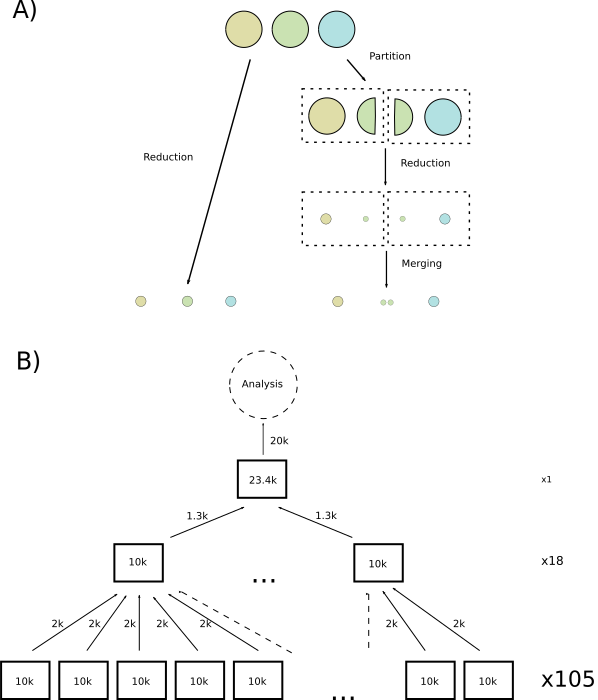
\includegraphics[width=\textwidth,height=\textheight,keepaspectratio]{pyproct_supp_compression.pdf}

\caption{A) Global reduction of the size of the dataset vs. merging local reductions. B) Different levels of compression including the number of frames used in each level.}
\label{fig:compression}
\end{figure}

The goal of this technique is to reduce the input trajectory by exchanging
sets of similar conformations (clusters) by a choice of its most representative
structures so that the final number of elements is proportional to
the original size of the cluster.

The first step to apply the reduction is to produce a clustering.
This makes us face the memory problem mentioned before. A workaround
for this issue is to divide the trajectory into smaller parts so that
each distance matrix can fit in memory, process each part separately
and then merge them again. Unfortunately, arbitrarily partitioning
the trajectory can separate elements that could form part of the same
cluster (which is more prone to happen in the boundaries of each part).
This can lead to an unevenness in the redundancy elimination process
(see the 2D example in Fig. \ref{fig:compression}A). We have performed
the reduction process iteratively to mitigate the problem. We start
with 105 parts of almost 10k frames each. After reducing each part
to 2k frames, we merged them into groups of 7 (\around14k
frames each). These groups were compressed to have around 1.3k frames
each and merged again to form a \around24k frames trajectory.
This was finally reduced to 20k frames and then analyzed. 


\subsubsection{Results}


\subsubsubsection{Performance}

pyProCT was run in an Intel Xeon CPU W3530 @ 2.80GHz workstation.
Each run of pyProCT spawned a maximum of 6 processes. While it was
being executed the workstation was normally used, occasionally triggering
operating system's swap mechanisms, which slowed down the process.
Therefore, the calculated execution time has merely a qualitative
meaning (see Table \ref{tab:results}). Also, the lack of knowledge of the
system forced us to use a very general hypothesis, increasing the
number of clusterings that had to be generated and thus the total
execution time. 

\begin{table}
\centering
\begin{tabular}{ r c c c }
\toprule
Level & Runs & Time per run (s) & Clusterings per run \\
\midrule

Third (10k$\rightarrow$2k) & 105 & \around1500 & 300-400\\
Second (20k$\rightarrow$1.3k) & 18 & \around2200 & 300-400\\
First (24k$\rightarrow$20k) & 1 & 12395 & 452\\
\bottomrule

\end{tabular}
\protect\caption{Around 40k clusterings were produced in almost 58h (1 clustering each
5s).\label{tab:results}}
\end{table}

\subsubsubsection{Clustering}

The clustering chosen by pyProCT was composed of a total of 19 clusters,
one of them holding the 34\% of the conformations. The C$\alpha$-RMSD
with the experimental structure (PDB id 2JOF) is 1.8${\AA}$, which
is similar to the 1.4${\AA}$ RMSD calculated in the original article
(see Fig. \ref{fig:clusters}). 

\begin{figure}
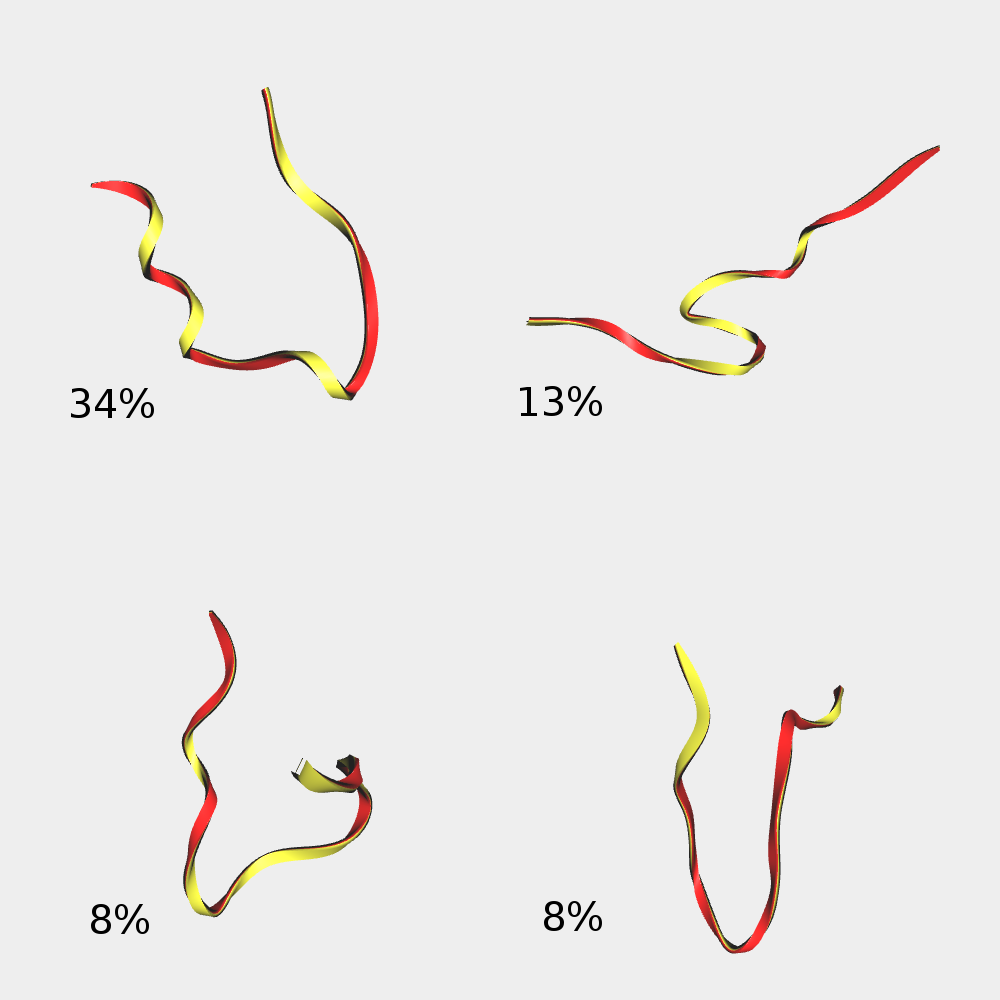
\includegraphics[width=\textwidth,height=\textheight,keepaspectratio]{pyproct_supp_clusters.png}

\protect\caption{Representative conformations for the 4 most populated clusters, holding
a 34\%, 13\%, 8 \% and 8\% of the elements of the dataset. \label{fig:clusters}}
\end{figure}


\subsection{2D Validation}
\label{sec:pyproct_supp_6}

In order to improve the reliability of pyProCT we have performed two
different quality assurance methods. The first was to ensure that
the software itself was working correctly using a unit testing methodology
(trying to get the best possible test coverage). The second was centered
in the validation of the clustering algorithms and the protocol.

Clusterings are hard to validate, especially when using
multidimensional data. Validating a 2D clustering, however, can be
an easier task as it can be visually checked. To this end we coded
the scripts that can be found in the folder\texttt{ pyproct/validation/bidimensional/}.


\subsubsection{Datasets}

To perform the validation, we downloaded some of Helmuth Spaeth's\cite{spaeth_spaeth_????-1}
datasets. These datasets have different characteristics that make them
difficult to cluster : 
\begin{enumerate}
	\item In this dataset 3 to 5 clusters can be seen. It looks like some of
	them can be subdivided. In general, these clusters are compact.
	\item It shows a set of points homogeneously covering the plane. There is not noticeable
	density variations.
	\item In this case there are two different density regions. In the bottom-right
	corner there is a compact cluster. The remaining points are sparsely
	distributed in the remaining space .
	\item Two compact clusters to the left, one big cluster (which seems to
	be composed of other clusters) sits on the right.
	\item Three parallel elongated clusters of different sizes and densities.
	\item Three elongated clusters with similar densities sharing the same origin.
	\item Two overlapped elongated clusters with different densities.
	\item Three elongate clusters with similar densities. All three are overlapped.
\end{enumerate}

We also used a code adapted from Jochen Wersdrfer's blog \cite{wersdorfer_spectral_????}
to generate a 9th dataset, which contains 450 points lying in three
concentric circles.


\subsubsection{Protocol validation}

In the first version of the validation script we used the datasets
to validate the algorithms, that is, we coded some algorithm-parameter
pairs and checked a picture of the resulting clusterings. Since the
algorithms were working as expected, we upgraded the script to fully
test the HCE protocol.

For each dataset, two hypotheses about the noise, cluster size and
number of clusters were defined (see \ref{tab:description_table})
based on our observations of the datasets. Also, we used two different
criteria to describe the expected clusterings:

\begin{description}
	\item [``default\_criteria''] Uses Silhouette and Cohesion ICVs. Is
	the default criteria of pyProCT and fosters both separation and compactness.
	\item [``graph\_criteria''] Uses the 'NCut' ICV. It tries to separate
	a graph representation of the dataset into connected components so
	that the sum of inner edge weights is optimized.
\end{description}

\begin{figure}
	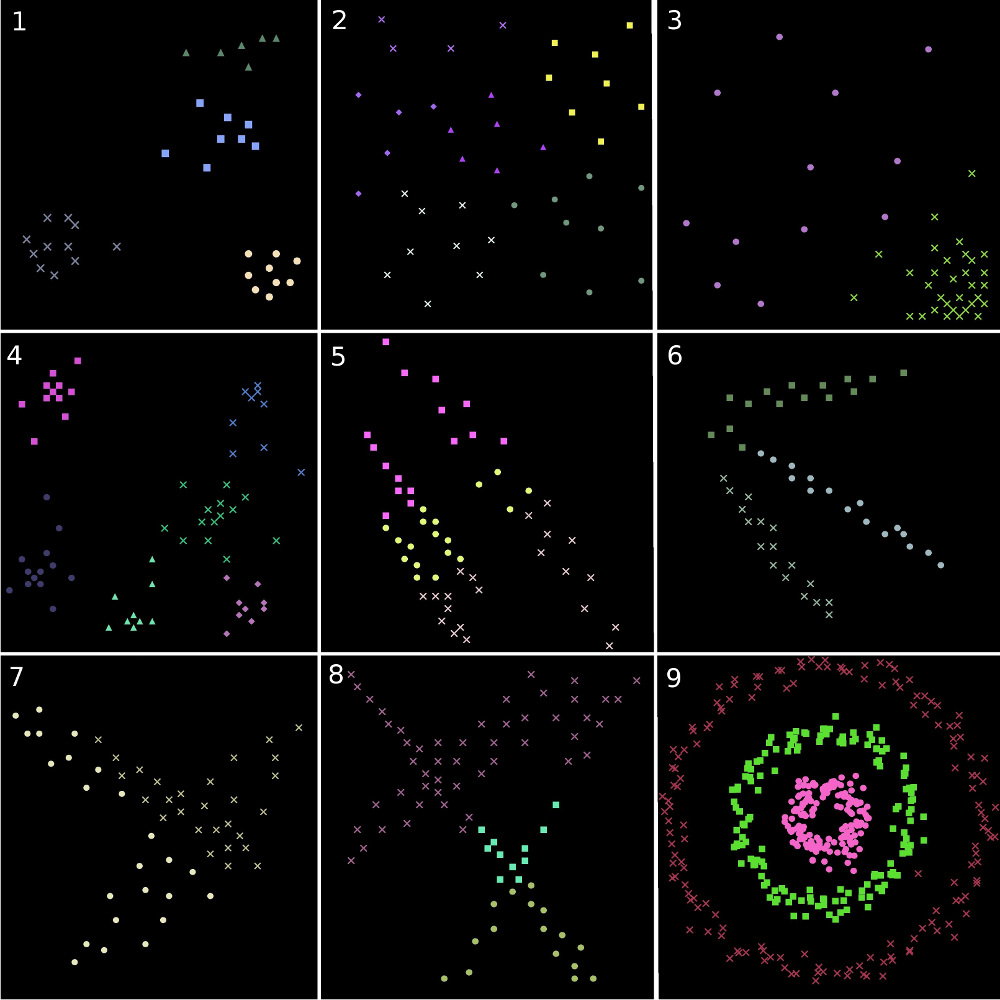
\includegraphics[width=\textwidth,height=\textheight,keepaspectratio]{pyproct_supp_c_plots}

	\protect\caption{Results of the application of pyProCT to nine 2D datasets. Clusters
	are plotted using different colors and symbols.\label{fig:plots_2d}}

\end{figure}

\begin{table}
\centering
\begin{tabular}{ c c c c c c }
\toprule
Dataset & \specialcell{Min.\\Clusters} & \specialcell{Max.\\Clusters} & \specialcell{Min.\\Cluster Size} & \specialcell{Max.\\Noise} & Criteria\\
\midrule
1 & 2 & 10 & 3 & 10\% & ``default\_criteria''\\
2 & 2 & 10 & 2 & 10\% & ``default\_criteria''\\
3 & 2 & 10 & 10 & 10\% & ``default\_criteria''\\
4 & 2 & 10 & 8 & 10\% & ``default\_criteria''\\
5 & 3 & 10 & 10 & 5\% & \specialcell{``default\_criteria'' \\ and ``graph\_criteria''}\\
6 & 3 & 10 & 13 & 10\% & ``graph\_criteria''\\
7 & 2 & 10 & 10 & 10\% & \specialcell{``default\_criteria'' \\ and ``graph\_criteria''}\\
8 & 3 & 8 & 5 & 10\% & \specialcell{``default\_criteria'' \\ and ``graph\_criteria''}\\
9 & 3 & 4 & 100 & 5\% & ``graph\_criteria''\\
\bottomrule
\end{tabular} \protect\caption{Clustering hypothesis for each of the datasets.\label{tab:description_table}}


\end{table}

\begin{figure}
	\fittopageimage{pyproct_supp_concentric_circles}

	\protect\caption{An incorrect choice of the ICVs to express the desired resulting clustering
	traits can drastically modify the results. In this case the criteria
	was changed from ``graph\_criteria'' to ``default\_criteria'',
	favoring one of the clusterings generated by the K-Medoids algorithm.
	\label{fig:concentric_circles}}
\end{figure}


\subsubsection{Results}

Clusterings 1, 3, 4, 6 and 9 are in full accordance with
our expectations (see table \ref{tab:results_table} and Fig. \ref{fig:plots_2d}).
We thought that the optimum solution for dataset 2 could be to use
one single cluster encompassing all elements. However the final partition
in 5 clusters looks reasonable. 

Clustering 5, 7 and 8 are different of what our intuition dictates.
The main problem that pyProCT has when dealing with a dataset like
7 or 8 is that their ``natural'' clusters overlap i.e. there are
elements that belong to more than one cluster at the same time. This
could be overcome by adding fuzzy algorithms to the algorithms pool.
Despite this, results would look counterintuitive in any case, as its usefulness
in most scenarios implies to discretize the membership values.

Clustering 5 highlights a weakness of the HCE methodology: its success
depends on the ability of the user to convey their goals in the clustering
hypothesis. If the user is not able to express it using pyProCT built-in
ICVs (see Fig. \ref{fig:concentric_circles}) or the needed ICVs to define
the hypothesis are not yet implemented, it would be impossible for
users to get the best-fitted result for their problems. It is clear
that, in this case, none of the used criteria suffices to choose the
type of result we would like to obtain.

\begin{table}
\centering
\begin{tabular}{ c c c c c }
\toprule
Dataset & Algorithm & Num. Clusters & Noise & Criteria\\
\midrule
1 & Gromos & 4 & 8.10\% & ``default\_criteria''\\
2 & Spectral Clust. & 5 & 0\% & ``default\_criteria''\\
3 & K-Medoids & 2 & 0\% & ``default\_criteria''\\
4 & K-Medoids & 6 & 9.59\% & ``default\_criteria''\\
5 & K-Medoids & 3 & 0\% & ``graph\_criteria''\\
6 & DBSCAN & 3 & 4\% & ``graph\_criteria''\\
7 & K-Medoids & 2 & 0\% & ``graph\_criteria''\\
8 & K-Medoids & 3 & 5.19\% & ``graph\_criteria''\\
9 & Spectral Clust. & 3 & 0\% & ``graph\_criteria''\\
\bottomrule
\end{tabular}

\protect\caption{Details of the results. Last column indicates the criteria
that obtained the best score. \label{tab:results_table}}
\end{table}


\newpage
\cleardoublepage
